\documentclass[aspectratio=169,professionalfonts, 12pt]{beamer}
\usepackage{lstbayes}
\usepackage[ruled]{algorithm}
\usepackage{algpseudocode,algorithmicx}
\usepackage{lmodern}
\usepackage{array}
\usepackage{multirow}
\usepackage[french,english]{babel}
\usepackage[T1]{fontenc}
\usepackage{multicol}
\usepackage{ragged2e}   %new code
\usepackage[utf8]{inputenc}
\usepackage[brazil]{varioref}
\usepackage[square,sort,comma,super,authoryear]{natbib}
\usepackage{listings,xcolor}
\usepackage{xmpmulti}
\usepackage{epsfig}
\usepackage{subcaption}
\captionsetup{compatibility=false}
\usepackage{ru,graphicx,hyperref,url} % 
\usepackage{booktabs}
\usepackage{pgfplots}
\usepackage{tikz}
\usepackage{ amsmath, amssymb, amsfonts}
\lstset{
    breaklines=true,
    %
    extendedchars=true,
    literate=
    {á}{{\'a}}1 {é}{{\'e}}1 {í}{{\'i}}1 {ó}{{\'o}}1 {ú}{{\'u}}1
    {Á}{{\'A}}1 {É}{{\'E}}1 {Í}{{\'I}}1 {Ó}{{\'O}}1 {Ú}{{\'U}}1
    {à}{{\`a}}1 {è}{{\`e}}1 {ì}{{\`i}}1 {ò}{{\`o}}1 {ù}{{\`u}}1
    {À}{{\`A}}1 {È}{{\'E}}1 {Ì}{{\`I}}1 {Ò}{{\`O}}1 {Ù}{{\`U}}1
    {ä}{{\"a}}1 {ë}{{\"e}}1 {ï}{{\"i}}1 {ö}{{\"o}}1 {ü}{{\"u}}1
    {Ä}{{\"A}}1 {Ë}{{\"E}}1 {Ï}{{\"I}}1 {Ö}{{\"O}}1 {Ü}{{\"U}}1
    {â}{{\^a}}1 {ê}{{\^e}}1 {î}{{\^i}}1 {ô}{{\^o}}1 {û}{{\^u}}1
    {Â}{{\^A}}1 {Ê}{{\^E}}1 {Î}{{\^I}}1 {Ô}{{\^O}}1 {Û}{{\^U}}1
    {œ}{{\oe}}1 {Œ}{{\OE}}1 {æ}{{\ae}}1 {Æ}{{\AE}}1 {ß}{{\ss}}1
    {ç}{{\c c}}1 {Ç}{{\c C}}1 {ø}{{\o}}1 {å}{{\r a}}1 {Å}{{\r A}}1
    {€}{{\EUR}}1 {£}{{\pounds}}1
}

\addtobeamertemplate{block begin}{}{\justifying}
\setbeamertemplate{section in toc}[sections numbered]
\AtBeginSection[]
{
  \begin{frame}[t]
  \begin{multicols}{2}
      \tableofcontents[currentsection]
    \end{multicols}
  \end{frame}

}

\date{\today}
\definecolor{blueforest}{RGB}{80,00,00}
\begin{document}
\selectlanguage{french}
\begin{frame}[plain, noframenumbering]
	\titlepage
\end{frame}
\begin{frame}[plain,t, noframenumbering]
	\frametitle{Table des matières}
    \begin{multicols}{2}
    \tableofcontents
    \end{multicols}
\end{frame}

% Section titles are shown in at the top of the slides with the current section 
% highlighted. Note that the number of sections determines the size of the top 
% bar, and hence the university name and logo. If you do not add any sections 
% they will not be visible.
\section{INTRODUCTION}

\subsection{Contexte}


\begin{frame}
  \frametitle{Contexte}
  \justifying
  \begin{minipage}{\textwidth}
    \begin{figure}[H]
      \centering
      \subfloat{{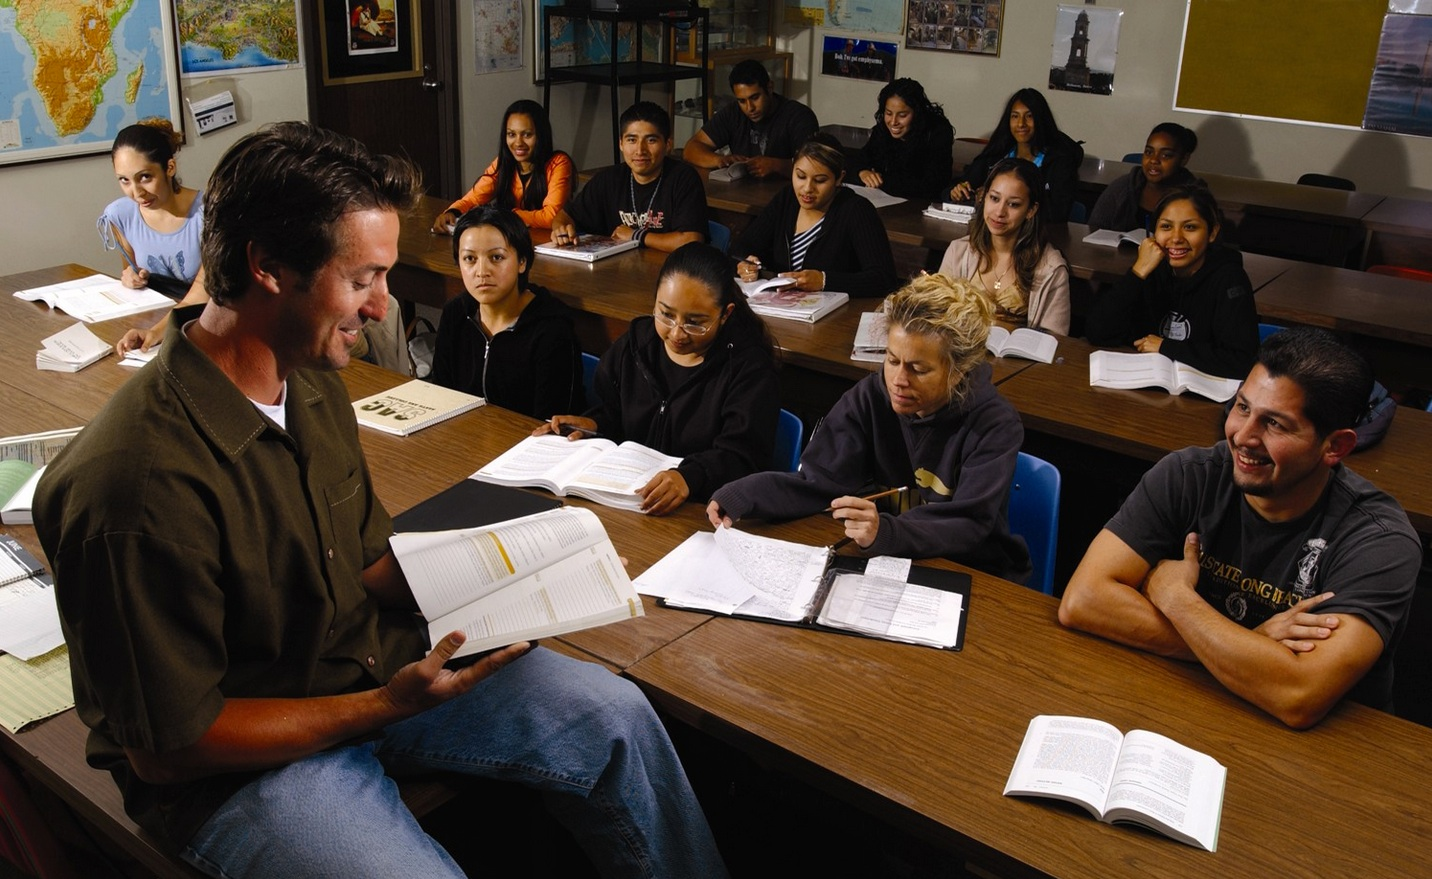
\includegraphics[width=7cm]{images/etat_art/face.jpg}}}%
      \qquad
      \subfloat{{
\includegraphics[width=6cm]{images/etat_art/elarning.jpg}}}%
      %\caption{Dendrogramme}%
    \end{figure}
  \end{minipage}
\end{frame}


\begin{frame}
  \frametitle{Introduction}
  \framesubtitle{Contexte}
  \begin{minipage}{0.5\textwidth}
    \begin{block}{Contexte(suite)}
    Les systèmes informatisés conservent des données détaillées des interactions utilisateur-système, plus précisément des interactions système-apprenant dans les systèmes éducatifs.
    \end{block}
    \only<1->
  \end{minipage}
  \begin{minipage}{2cm}
  
  \end{minipage}
  \begin{minipage}{0.4\textwidth}
    \begin{figure}[t]
    \begin{center}
      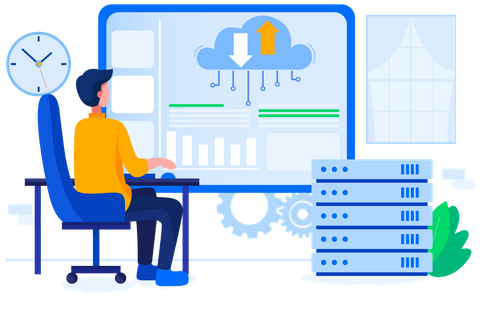
\includegraphics[width=\textwidth]{images/etat_art/database_illustration.png}
    \end{center}
    \end{figure} 
  \end{minipage}
\end{frame}

\begin{frame}
  \frametitle{Introduction}
  \framesubtitle{Contexte}
  \begin{minipage}{0.5\textwidth}
    \begin{block}{Contexte(suite)}
    Ces données détaillées qui sont dans une grande base de données offrent des opportunités pour étudier ces données récolter.  
    \end{block}
  \end{minipage}
  \begin{minipage}{2cm}
  
  \end{minipage}
  \begin{minipage}{0.4\textwidth}
    \begin{figure}[t]
    \begin{center}
      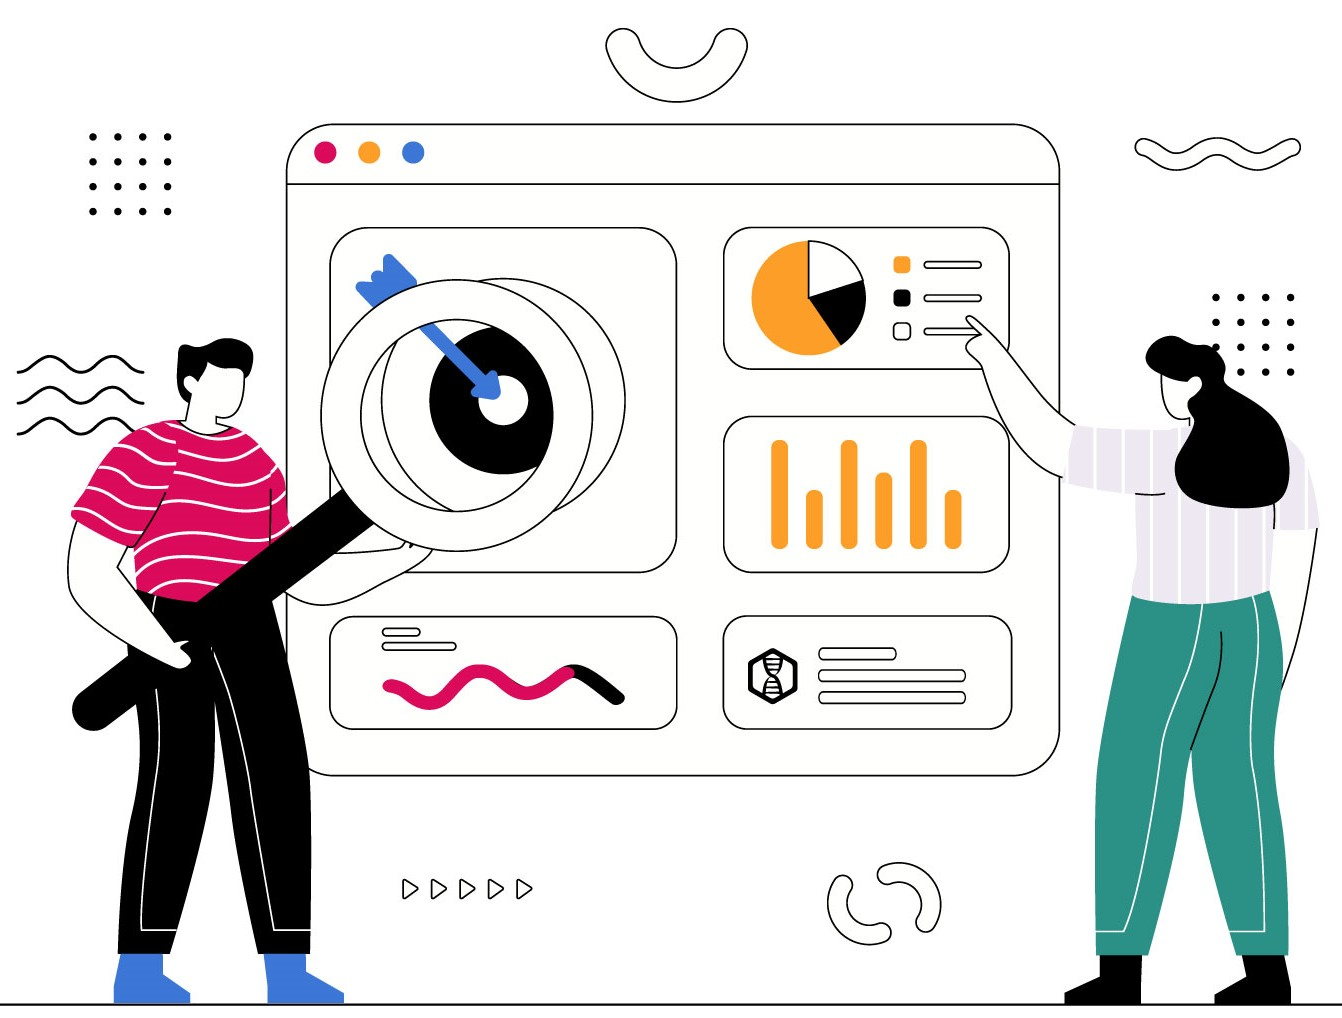
\includegraphics[width=\textwidth]{images/etat_art/data_oppor.jpeg}
    \end{center}
    \end{figure} 
  \end{minipage}
\end{frame}


\subsection{Problématique}

\begin{frame}
  \frametitle{Introduction}
  \framesubtitle{Problématique}
  \justifying
  \begin{alertblock}{Problèmes}
  Cependant les données ne sont jamais aussi complètes et sans équivoque qu’elles garantissent la certitude. \\
  Aussi, dans les systèmes éducatifs, beaucoup d’aptitudes ont une forte relation causale dans laquelle une aptitude doit être présentée avant une autre.
\end{alertblock}
\end{frame}

\begin{frame}
  \frametitle{Introduction}
  \framesubtitle{Problématique}
  \begin{minipage}{0.5\textwidth}
    \begin{alertblock}{Problèmes \(\displaystyle \blacktriangleright \) 1}
      Cependant les données ne sont jamais aussi complètes et sans équivoque qu’elles garantissent la certitude.
    \end{alertblock}
    \only<1->
  \end{minipage}
  \begin{minipage}{2cm}
  
  \end{minipage}
  \begin{minipage}{0.4\textwidth}
    \begin{figure}[t]
    \begin{center}
      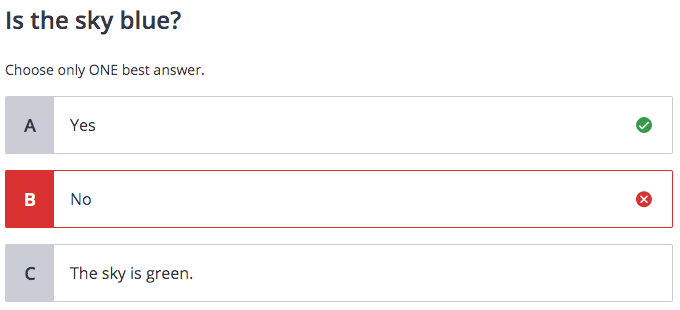
\includegraphics[width=\textwidth]{images/etat_art/quiz_response1_1.png}
    \end{center}
    \end{figure} 
  \end{minipage}
\end{frame}

\begin{frame}
  \frametitle{Introduction}
  \framesubtitle{Problématique}
  \begin{minipage}{\textwidth}
    \begin{alertblock}{Problèmes \(\displaystyle \blacktriangleright \) 2}
      Aussi, dans les systèmes éducatifs, beaucoup d’aptitudes ont une forte relation causale dans laquelle une aptitude doit être présentée avant une autre.
    \end{alertblock}
  \end{minipage}

  \begin{minipage}{\textwidth}
    \begin{figure}[t]
    \begin{center}
      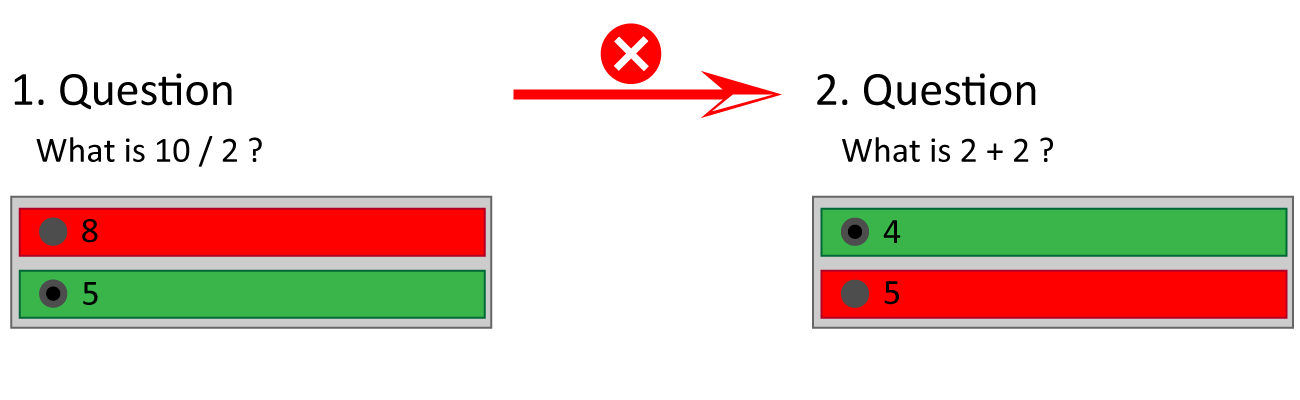
\includegraphics[width=\textwidth]{images/etat_art/hierarchi_competence2.png}
    \end{center}
    \end{figure} 
  \end{minipage}
\end{frame}

\begin{frame}
  \frametitle{Introduction}
  \framesubtitle{Problématique}
  \begin{minipage}{\textwidth}
    \begin{alertblock}{Problèmes \(\displaystyle \blacktriangleright \) 2}
      Aussi, dans les systèmes éducatifs, beaucoup d’aptitudes ont une forte relation causale dans laquelle une aptitude doit être présentée avant une autre.
    \end{alertblock}
  \end{minipage}

  \begin{minipage}{\textwidth}
    \begin{figure}[t]
    \begin{center}
      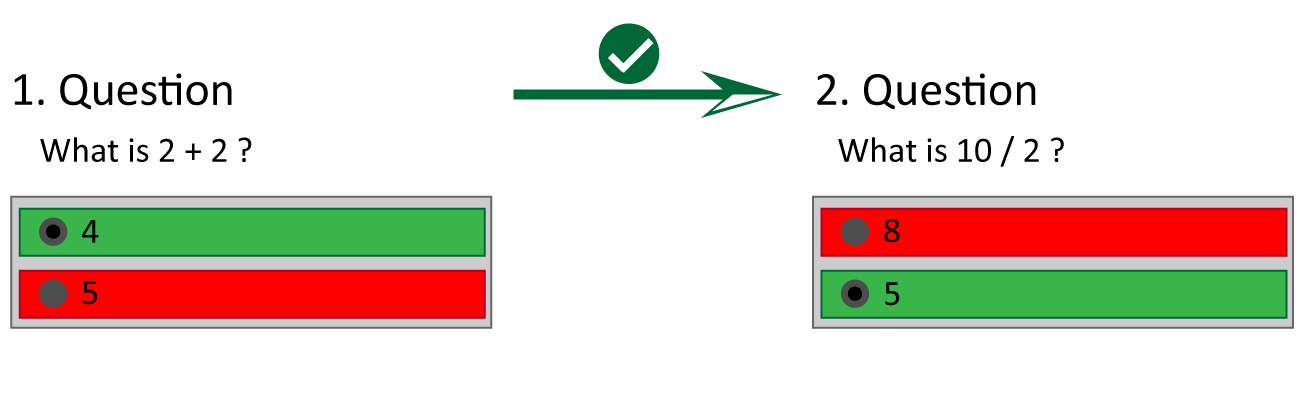
\includegraphics[width=\textwidth]{images/etat_art/hierarchi_competence.png}
    \end{center}
    \end{figure} 
  \end{minipage}
\end{frame}


\subsection{Objectif}

\begin{frame}
  \frametitle{Objectif}
  \begin{block}{L'objectif principal}
    Analyse et évaluation du jeu de données en faisant un ajustement bayésien des réponses aux items avant de décider si oui ou non le jeu de données valle le coup d’être utilisé.\\
    Après la validation du jeu de données, les items sont regroupés en composante de connaissance en utilisant une approche basée sur la similarité qui utilise une matrice de similarité calculée selon quatre catégories : réponse correcte et incorrecte avec aide et sans aide.
  \end{block}     
\end{frame}

\begin{frame}
  \frametitle{Introduction}
  \framesubtitle{Objectif}
  \begin{minipage}{0.4\textwidth}
    \begin{block}{L'objectif principal}
      Après la validation du jeu de données, les items sont regroupés en composante de connaissance en utilisant une approche basée sur la similarité qui utilise une matrice de similarité calculée selon quatre catégories : réponse correcte et incorrecte avec aide et sans aide.
    \end{block} 
    \only<1->
  \end{minipage}
  \begin{minipage}{2cm}
  
  \end{minipage}
  \begin{minipage}{0.5\textwidth}
    \begin{figure}[t]
    \begin{center}
      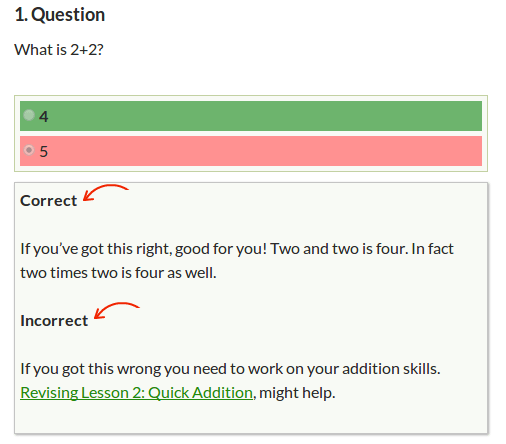
\includegraphics[width=\textwidth]{images/etat_art/quiz_response2.png}
    \end{center}
    \end{figure} 
  \end{minipage}
\end{frame}

\section{APERÇU SUR L'\'ETAT DE L'ART}
\subsection{Educational data minig}

\begin{frame}
  \frametitle{Aperçu sur l'état de l'art}
  \framesubtitle{Educational data minig}
  \justifying 
  \begin{minipage}{\textwidth}
  \begin{block}{}
    L’exploration de données est un processus visant à découvrir des modèles de données dans de grandes bases de données. Appliquer dans l’éducation, les données proviennent du milieu éducatif et le but principal est de comprendre le comportement des apprenants et l’environnement de leur apprentissage.  
  \end{block}
  \end{minipage}
\end{frame}

\begin{frame}
  \frametitle{Aperçu sur l'état de l'art}
  \framesubtitle{Educational data minig}
  \justifying 
  \begin{minipage}{\textwidth}
  \begin{figure}[H]
      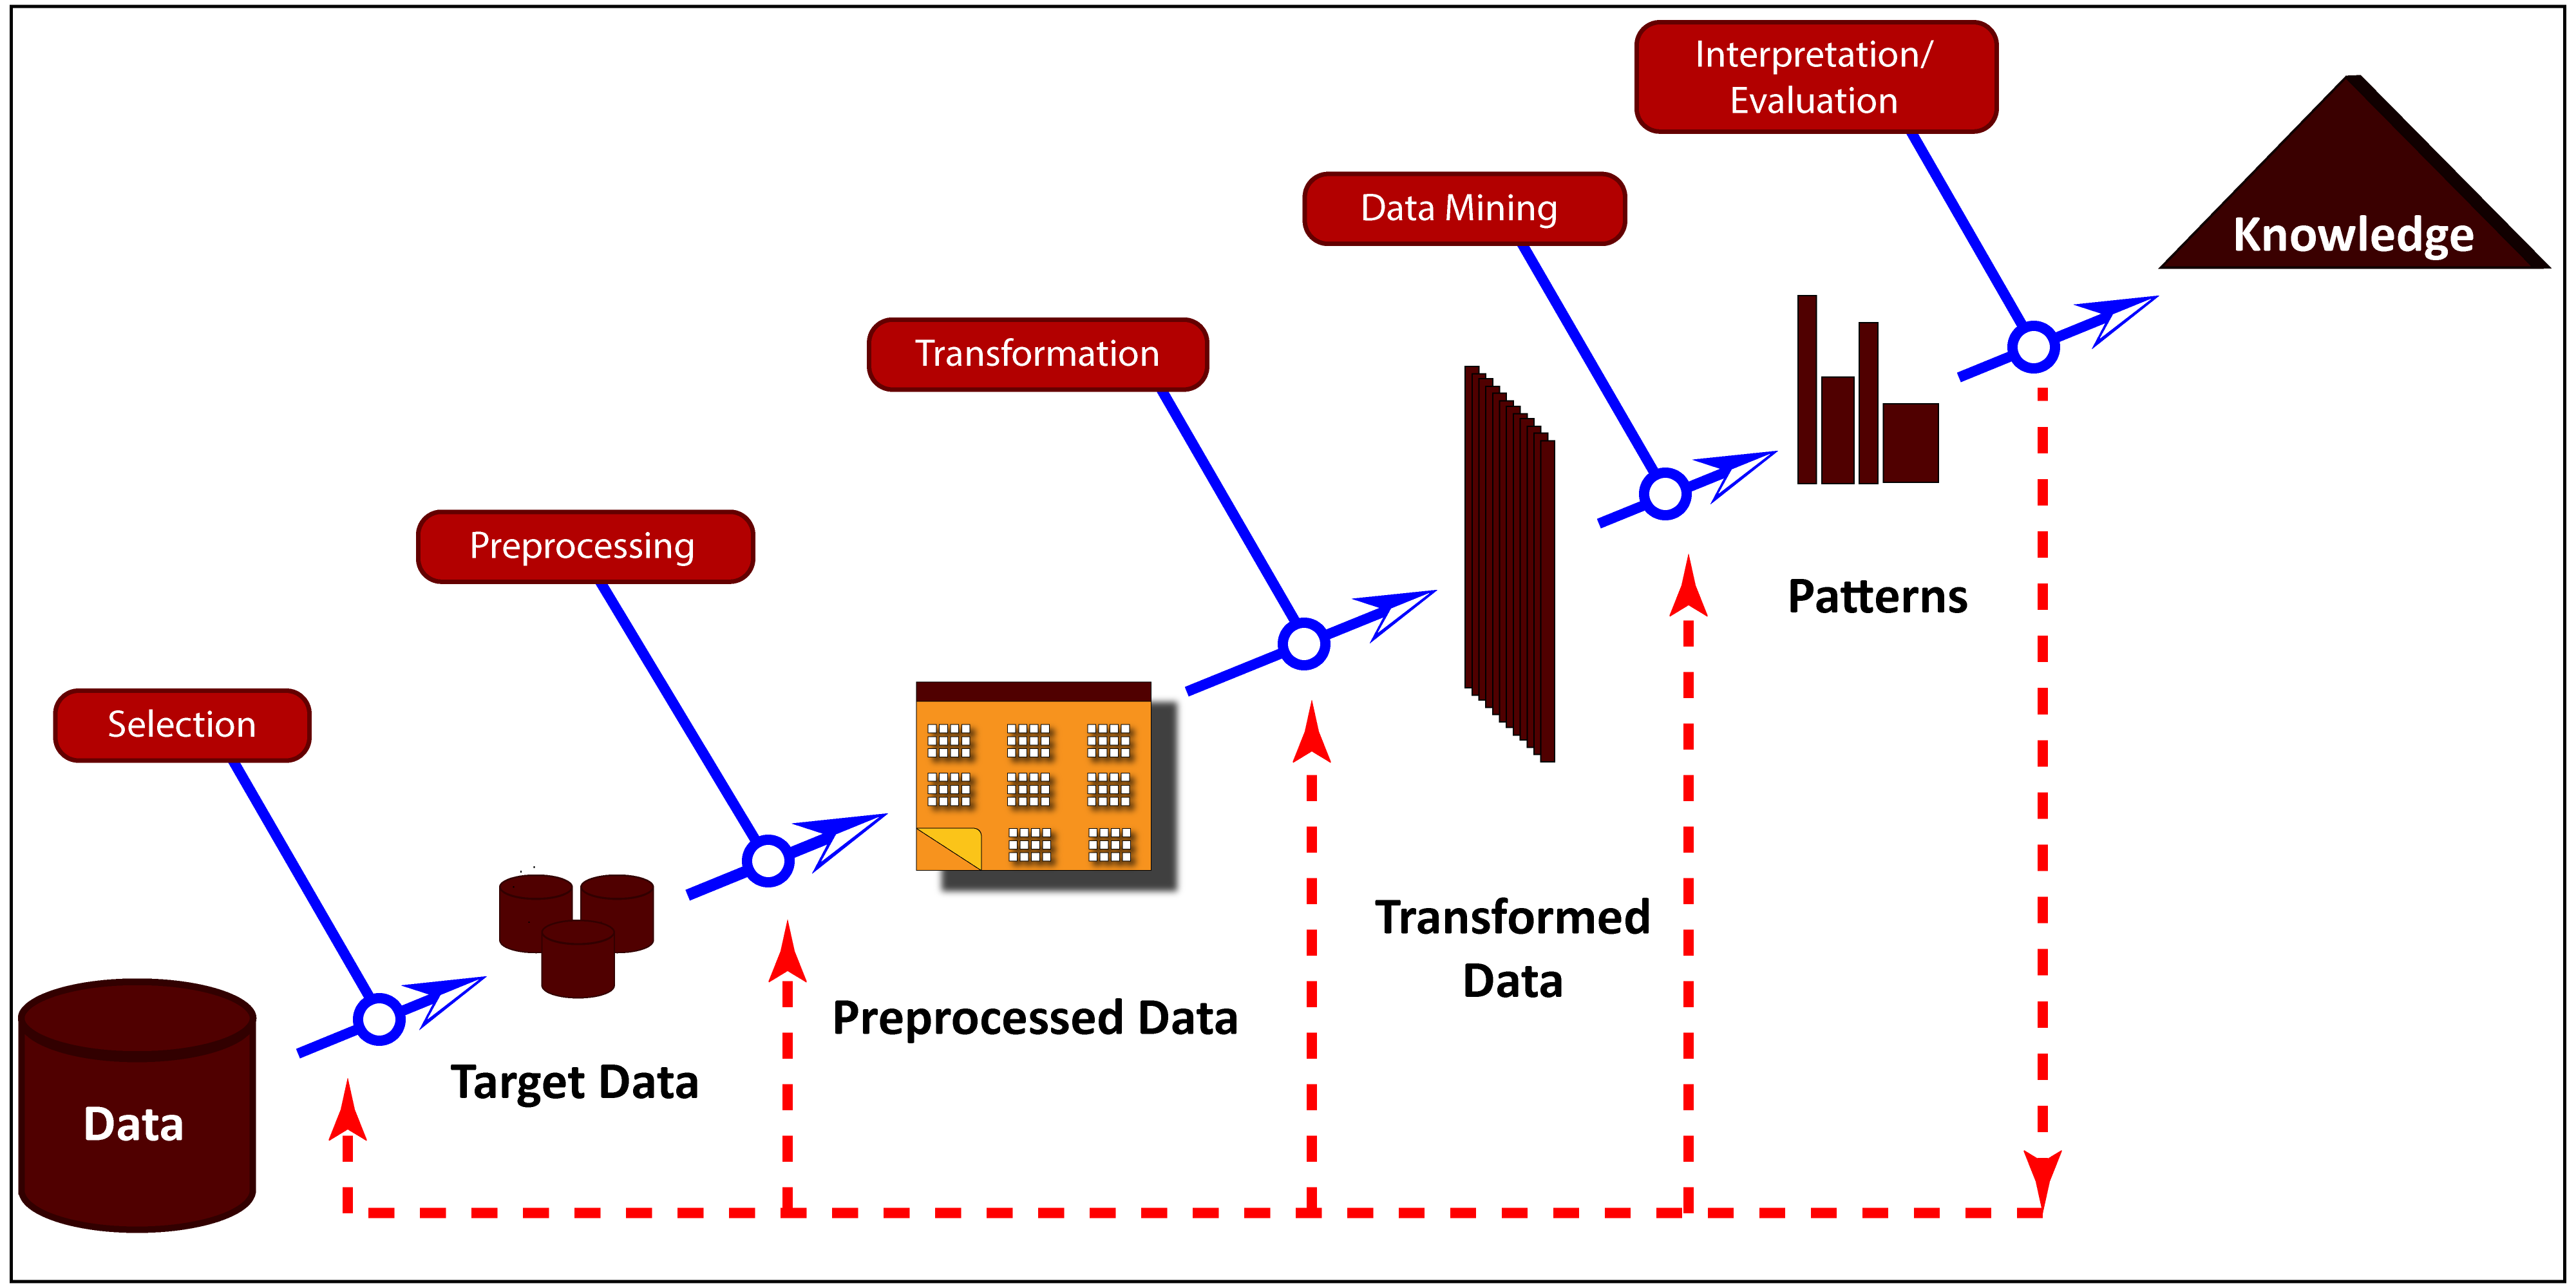
\includegraphics[height=6cm]{images/etat_art/extract_data_steps.png}
  \end{figure}
  \end{minipage}
\end{frame}


\subsection{Modèle de l’apprenant}

\begin{frame}
  \frametitle{Aperçu sur l'état de l'art}
  \framesubtitle{Modèle de l’apprenant}
  \justifying 
  \begin{minipage}{\textwidth}
  \begin{block}{Définition}
    Le modèle de l’apprenant est une structure de données qui reflète l’état des connaissances supposées de l’apprenant sur un domaine cible.
  \end{block}
    \only<1->
  \end{minipage} 
  \begin{minipage}{\textwidth}
  \onslide<2->
  \begin{block}{}
    Quelque catégorie du modèle de l’apprenant :
    \begin{itemize}
      \item Modèle cognitif,
      \item Modèle d’inférence,
      \item Modèle émotionnel.
    \end{itemize}
  \end{block}
  \end{minipage}
\end{frame}

\begin{frame}
  \frametitle{Aperçu sur l'état de l'art}
  \framesubtitle{Modèle de l’apprenant}
  \justifying 
  \begin{minipage}{\textwidth}
  \begin{block}{Le modèle cognitif}
    La modélisation cognitive est utilisé pour simuler ou prédire le comportement humain ou les performances sur des tâches similaires à celles modélisées et améliorer l'interaction homme-machine.  \end{block}
  \only<1->
  \end{minipage} 
  % \begin{minipage}{\textwidth}
  %   \begin{figure}[H]
  %     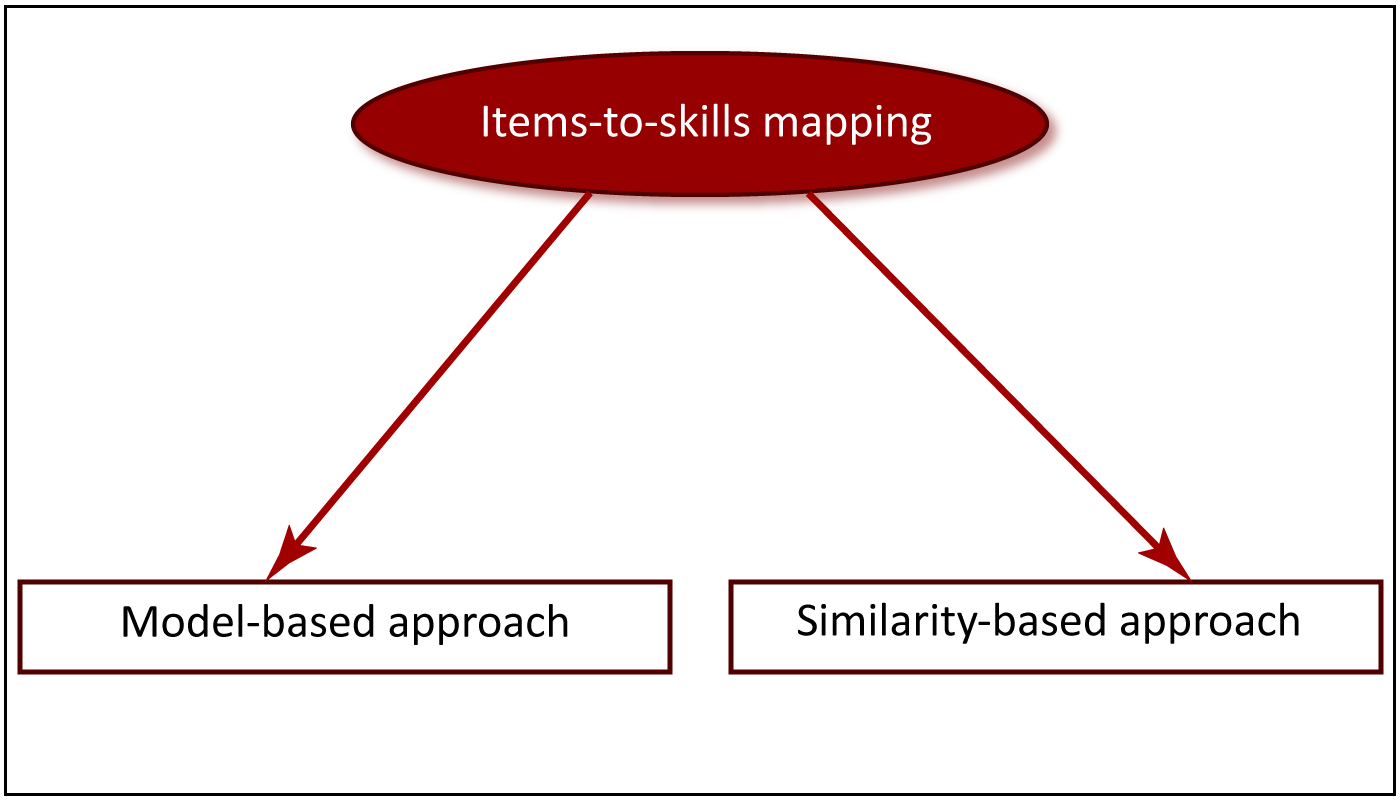
\includegraphics[ height=3.6cm]{images/etat_art/Items_mapping_structure.png}
  %   \end{figure}
  % \end{minipage}
\end{frame}

\begin{frame}
  \frametitle{Aperçu sur l'état de l'art}
  \framesubtitle{Modèle de l’apprenant}
  \justifying 
  \begin{minipage}{\textwidth}
  \begin{block}{Le modèle d’inférence}
    Cette approche est une sorte de moteur d’inférence qui fonctionne pour ajuster le modèle de l’apprenant. Il contient des règles qui lui permettent de raisonner sur le modèle cognitif et sur le modèle psychologique pour inférer de nouvelles connaissances dans le modèle de l’apprenant.  
  \end{block}
  \end{minipage} 
\end{frame}

\subsection{Analyse des items}

\begin{frame}
  \frametitle{Analyse des items}
  \justifying 
  \begin{minipage}{\textwidth}
  \begin{figure}[H]
      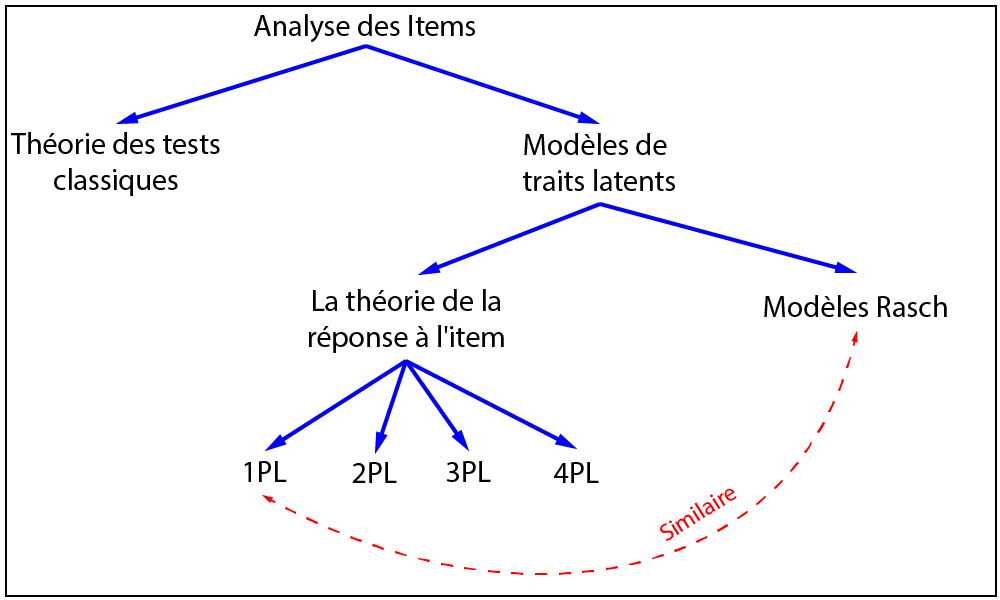
\includegraphics[height=6cm]{images/etat_art/items_analysis.png}
  \end{figure}
  \end{minipage}
\end{frame}

% \begin{frame}
%   \frametitle{Analyse des items}
%   \justifying 
%   \begin{minipage}{\textwidth}
%   \begin{figure}[H]
%       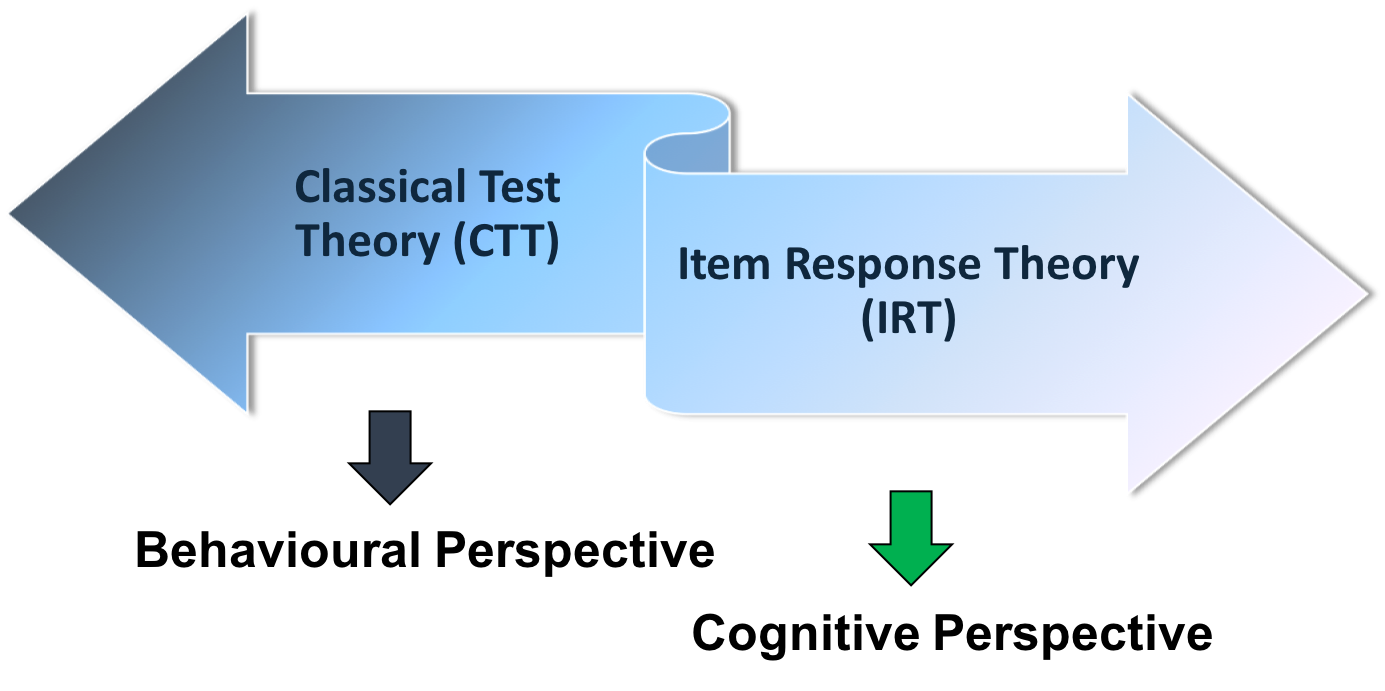
\includegraphics[height=6cm]{images/etat_art/ctt_irt.png}
%   \end{figure}
%   \end{minipage}
% \end{frame}

% \begin{frame}
%   \frametitle{Analyse des items}
%   \framesubtitle{Quelque définitions}
%   \justifying 
%   \begin{minipage}{\textwidth}
%   \begin{block}{}
%     La théorie de la réponse à l'item fait référence aux modèles mathématiques qui tentent d'expliquer la relation entre les traits latents et leurs manifestations.
%   \end{block}
%   \end{minipage} 
% \end{frame}

% \begin{frame}
%   \frametitle{Analyse des items}
%   \framesubtitle{Théorie des tests classiques}
%   \justifying 
%   \begin{minipage}{\textwidth}
%   \begin{block}{Théorie des tests classiques}
%     \begin{itemize}
%       \item	Les analyses sont la forme d'analyse la plus simple et la plus largement utilisée. Les statistiques peuvent être calculées par des progiciels statistiques facilement disponibles (ou même à la main).
%       \item	Les analyses classiques sont effectuées sur le test dans son ensemble plutôt que sur l'item et bien que des statistiques d'items puissent être générées, elles ne s'appliquent qu'à ce groupe d'étudiants sur cette collection d'items. 
%     \end{itemize}
%   \end{block}  
%   \end{minipage} 
% \end{frame}

\begin{frame}
  \frametitle{Analyse des items}
  \framesubtitle{Modèles de traits latents}
  \justifying 
  \begin{minipage}{\textwidth}
  \begin{block}{Modèles de traits latents}
    \begin{itemize}
      \item	Ils visent à mesurer la capacité sous-jacente qui produit la performance du test plutôt que de mesurer la performance en soi.
      \item	Cela les conduit à être sans échantillon. Comme les statistiques ne dépendent pas de la situation de test qui les a générées, elles peuvent être utilisées de manière plus flexible.
    \end{itemize}
  \end{block}  
  \end{minipage} 
\end{frame}

% \begin{frame}
%   \frametitle{Analyse des items}
%   \framesubtitle{Différence entre CTT et IRT.}
%   \justifying 
%   \begin{minipage}{\textwidth}
%   \begin{block}{Théorie des tests classiques vs modèles de traits latents}
%     \begin{itemize}
%       \item	L'analyse classique a pour base le test (pas l'item). Bien que les statistiques générées soient souvent généralisées à des étudiants similaires passant un test similaire ; ils ne s'appliquent vraiment qu'aux étudiants qui passent ce test.
%       \item	Les modèles de traits latents visent à regarder au-delà des traits sous-jacents qui produisent les performances du test. Ils sont mesurés au niveau de l'article et fournissent une mesure sans échantillon.  
%     \end{itemize}
%   \end{block}  
%   \end{minipage} 
% \end{frame}


% \begin{frame}
%   \frametitle{Analyse des items}
%   \framesubtitle{Avantages de l'IRT}
%   \justifying 
%   \begin{minipage}{\textwidth}
%   \begin{block}{Avantages de l'IRT}
%     \begin{itemize}
%       \item	Fournit plus d'informations que la théorie des tests classique (CTT).
%       \begin{itemize}
%         \item Les statistiques des tests classiques dépendent de l'ensemble des éléments et de l'échantillon examinés.
%         \item	Modélisation IRT indépendante de l'échantillon examiné.
%       \end{itemize}
%       \item Utilisé pour estimer les paramètres des éléments (par exemple, la difficulté et la discrimination).
%       \item Les vrais scores de l'apprenant sur le trait latent.
%     \end{itemize}
%   \end{block}  
%   \end{minipage} 
% \end{frame}

\begin{frame}
  \frametitle{Analyse des items}
  \framesubtitle{Modèle de Rasch}
  \justifying 
  \begin{minipage}{\textwidth}
  \begin{block}{Modèle de Rasch}
    Le modèle de Rasch est une méthode d'analyse de données statistiques pour mesurer des éléments tels que les capacités, les attitudes ou des traits de personnalité de personnes répondant à des questionnaires. 
  \end{block}  
  \end{minipage} 
\end{frame}


\begin{frame}
  \frametitle{Analyse des items}
  \framesubtitle{Modèle de Rasch}
  \justifying 
  \begin{minipage}{\textwidth}
    \centering \textbf{\underline{Structure de données typiques}}
    \begin{table}[H]
      \centering
      \begin{tabular}{|m{0.5cm}|m{0.5cm}|m{0.5cm}|m{0.5cm}|m{0.5cm}|} \hline
       & \textbf{I1} & \textbf{I2} & \textbf{I3} & \textbf{I4} \\ \hline
       \textbf{S1} & 0 & 0 & 1 & 1 \\ \hline
       \textbf{S2} & 0 & 1 & 1 & 1 \\ \hline
       \textbf{S3} & 1 & 1 & 1 & 1 \\ \hline
       \textbf{S4} & 0 & 0 & 0 & 0 \\ \hline
       \textbf{S5} & 0 & 0 & 1 & 0 \\ \hline
      \end{tabular}
      \hfill
      \begin{tabular}{|m{0.5cm}|m{0.5cm}|m{0.5cm}|m{0.5cm}|m{0.5cm}|} \hline
        & \textbf{I1} & \textbf{I2} & \textbf{I3} & \textbf{I4} \\ \hline
        \textbf{S4} & 0 & 0 & 0 & 0 \\ \hline
        \textbf{S5} & 1 & 0 & 0 & 0 \\ \hline
        \textbf{S1} & 1 & 1 & 0 & 0 \\ \hline
        \textbf{S2} & 1 & 1 & 1 & 0 \\ \hline
        \textbf{S3} & 1 & 1 & 1 & 1 \\ \hline
       \end{tabular}
    \end{table}
  \end{minipage} 
\end{frame}

\begin{frame}
  \frametitle{Analyse des items}
  \framesubtitle{Modèle de Rasch}
  \centering \textbf{\underline{Modèle de Guttman}} \\
  \justifying 
  \begin{minipage}{\textwidth}
    \begin{figure}
      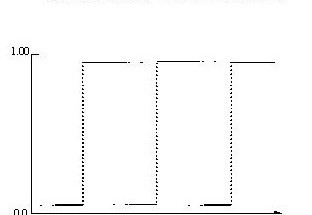
\includegraphics[width=0.475\textwidth]{images/etat_art/guttman_model.jpg}
   \end{figure}
  \end{minipage} 
\end{frame}

\begin{frame}
  \frametitle{Analyse des items}
  \framesubtitle{Le modèle probabiliste de Rasch}
  \justifying 
  \begin{minipage}{\textwidth}
  \begin{block}{La fonction logistique du modèle de Rasch}
  \begin{equation}P(x_{j}| \theta, \beta_{j}) = \frac{\exp \left[\theta - \beta_{j} \right]  }{1+ \exp \left[ \theta - \beta_{j} \right] }
  \end{equation}
  Où, \\
  \begin{itemize}
    \item[$\blacklozenge$] \(\displaystyle \theta \) la capacité, la compétence de l'apprenant 
    \item[$\blacklozenge$] \(\displaystyle \beta \) difficulté de l'item
  \end{itemize}
  \end{block}  
  \end{minipage} 
\end{frame}

\begin{frame}
  \frametitle{Analyse des items}
  \framesubtitle{Le modèle probabiliste de Rasch}
  \justifying 
  \begin{minipage}{\textwidth}
  \begin{figure}[H]
      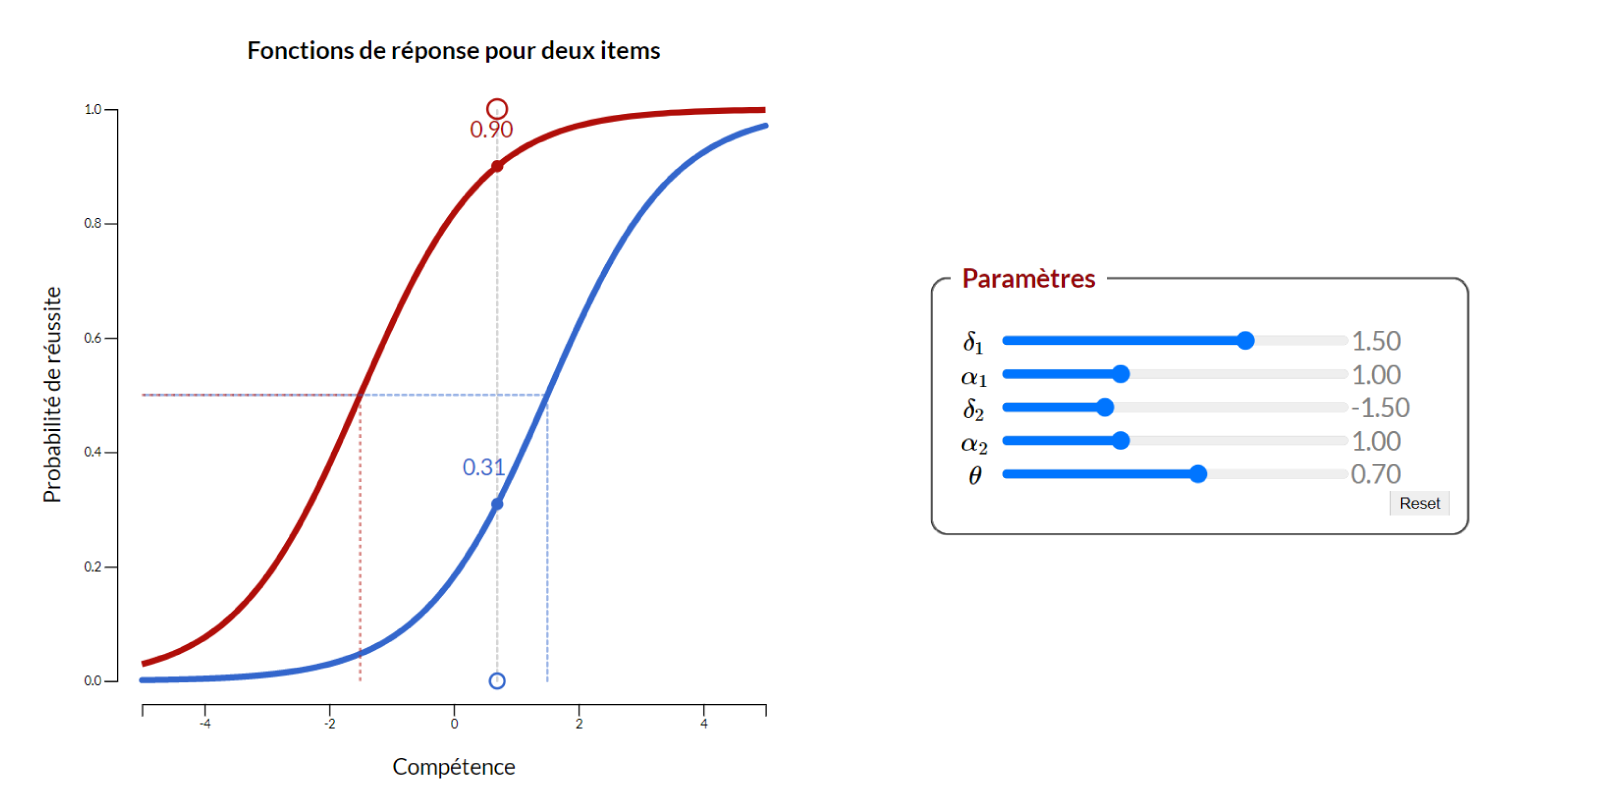
\includegraphics[height=6cm]{images/etat_art/rasch_figure.png}
  \end{figure}
  \end{minipage}
\end{frame}


\begin{frame}
  \frametitle{Analyse des items}
  \framesubtitle{La Théorie de la réponse à l'item}
  \justifying
  \begin{minipage}{\textwidth}
  \begin{block}{Modèle logistique à un paramètre}
    \begin{equation}
      P_{i}(\theta_{j} | X=1) = \frac{\exp \left[ 1.7 \alpha_{i}(\theta_{j}-\beta_{i}) \right]  }{1+ \exp \left[1.7 \alpha_{i}(\theta_{j}-\beta_{i}) \right]  } 
    \end{equation}
    Où, \\
    \begin{itemize}
      \item[$\blacklozenge$] \(\displaystyle \theta \) la capacité, la compétence de l'apprenant 
      \item[$\blacklozenge$] \(\displaystyle \beta \) paramètre de difficulté de l'item
      \item[$\blacklozenge$] \(\displaystyle \alpha \) paramètre de discrimination de l'item (fixe)
      \item[$\blacklozenge$] 1.7 facteur d'échelle 
    \end{itemize}
  \end{block}  
  \end{minipage} 
\end{frame}

\begin{frame}
  \frametitle{Analyse des items}
  \framesubtitle{La Théorie de la réponse à l'item}
  \justifying
  \begin{minipage}{\textwidth}
  \begin{block}{Modèle logistique à deux paramètres}
    \begin{equation}
      P_{i}(\theta_{j} | X=1) = \frac{\exp \left[ \alpha_{i}(\theta_{j}-\beta_{i}) \right]  }{1+ \exp \left[ \alpha_{i}(\theta_{j}-\beta_{i}) \right]  } 
    \end{equation}
    Où, \\
    \begin{itemize}
      \item[$\blacklozenge$] \(\displaystyle \theta \) la capacité, la compétence de l'apprenant 
      \item[$\blacklozenge$] \(\displaystyle \beta \) paramètre de difficulté de l'item
      \item[$\blacklozenge$] \(\displaystyle \alpha \) paramètre de discrimination de l'item(non fixe, peut changer par item)
    \end{itemize}
  \end{block}  
  \end{minipage} 
\end{frame}

\begin{frame}
  \frametitle{Analyse des items}
  \justifying 
  \begin{minipage}{\textwidth}
  \begin{figure}[H]
      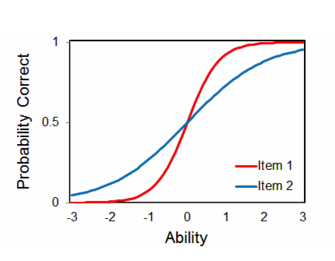
\includegraphics[height=6cm]{images/etat_art/2pl.png}
  \end{figure}
  \end{minipage}
\end{frame}

\begin{frame}
  \frametitle{Analyse des items}
  \framesubtitle{La Théorie de la réponse à l'item}
  \justifying
  \begin{minipage}{\textwidth}
  \begin{block}{Modèle logistique à trois paramètres}
    \begin{equation}
      P_{i}(\theta_{j}) = c_{i} +  \frac{1 - c_{i}}{1+ \exp \left[ -\alpha_{i}(\theta_{j}-\beta_{i}) \right]  } 
    \end{equation}
    Où, \\
    \begin{itemize}
      \item[$\blacklozenge$] \(\displaystyle \theta \) la capacité, la compétence de l'apprenant 
      \item[$\blacklozenge$] \(\displaystyle \beta \) paramètre de difficulté de l'item
      \item[$\blacklozenge$] \(\displaystyle \alpha \) paramètre de discrimination de l'item(non fixe, peut changer par item)
      \item[$\blacklozenge$] \(\displaystyle c \) paramètre de devinette.
    \end{itemize}
  \end{block}  
  \end{minipage} 
\end{frame}

\begin{frame}
  \frametitle{Analyse des items}
  \justifying 
  \begin{minipage}{\textwidth}
  \begin{figure}[H]
      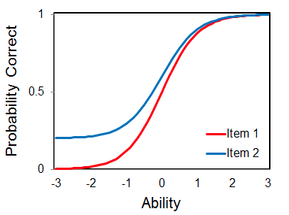
\includegraphics[height=6cm]{images/etat_art/IRT3.png}
  \end{figure}
  \end{minipage}
\end{frame}


\subsection{Inférence bayésienne}

\begin{frame}
  \frametitle{Inférence bayésienne}
  \begin{minipage}{0.4\textwidth}
    \begin{block}{Définition}
      L’inférence bayésienne est une méthode d’apprentissage des valeurs des paramètres dans les modèles statistiques à partir de données. 
    \end{block}
  \end{minipage}
  \begin{minipage}{2cm}
  
  \end{minipage}
  \begin{minipage}{0.5\textwidth}
    \begin{figure}[t]
    \begin{center}
      
\includegraphics[width=\textwidth]{images/etat_art/predire_inferer.png}
    \end{center}
    \end{figure} 
  \end{minipage}	
\end{frame}

\begin{frame}
  \frametitle{Inférence bayésienne}
  \begin{minipage}{0.6\textwidth}
  \begin{block}{Probabilité conditionnelle}
    La probabilité conditionnelle est la probabilité d'un événement sachant qu'un autre événement a eu lieu.\\
    Soit \(\displaystyle A \)  et \(\displaystyle B \) deux évènements avec \(\displaystyle P(A) \neq 0 \).
    \begin{equation}
      P(B|A) = \frac{P(A\cap B)}{P(A)}
      \label{conditionnelle_probability}
    \end{equation}
  \end{block}
  \end{minipage}
  \begin{minipage}{2cm}
  
  \end{minipage}
  \begin{minipage}{0.3\textwidth}
    \begin{figure}[t]
    \begin{center}
      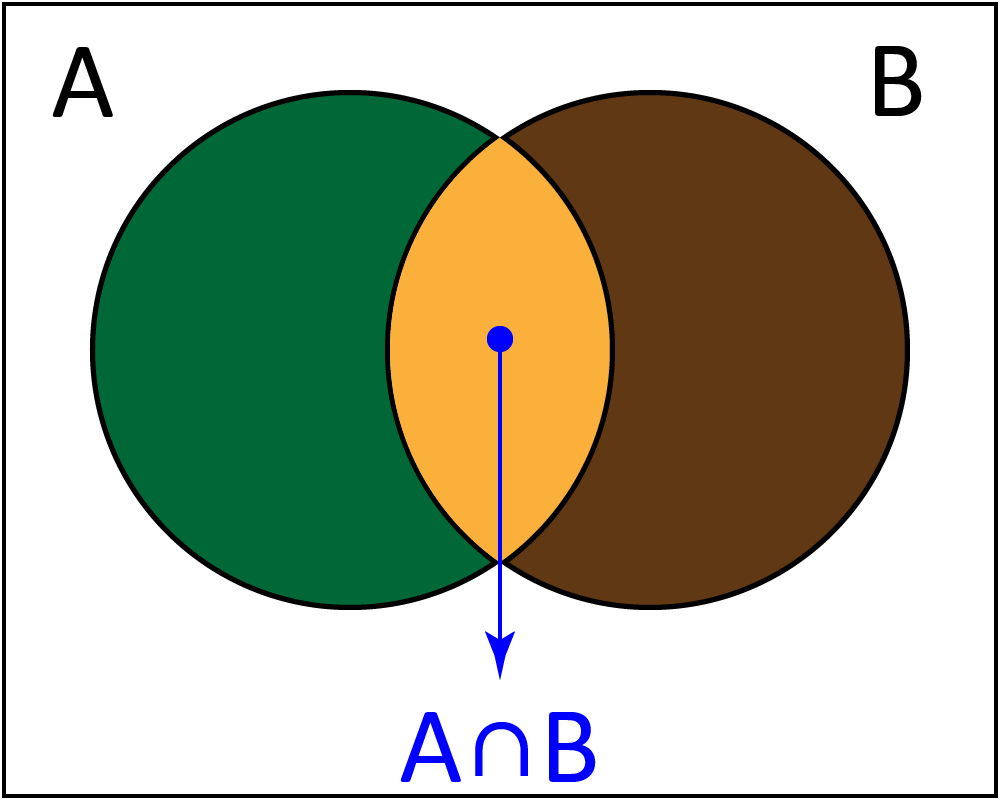
\includegraphics[width=\textwidth]{images/etat_art/conditional_b.png}
    \end{center}
    \end{figure} 
  \end{minipage}	
\end{frame}

\begin{frame}
  \frametitle{Inférence bayésienne}
  \justifying 
  \begin{minipage}{\textwidth}
  \begin{block}{Théorème de bayes}
    Le théorème de Bayes , du nom du mathématicien britannique du XVIIIe siècle Thomas Bayes est definit par l'équation suivante:   
    \begin{equation}
      Pr(B|A) = \frac{P(A\cap B)}{P(A)} = \frac{Pr(A|B)*Pr(B)}{Pr(A)}
      \label{theoreme_bayes}
    \end{equation} 
    \begin{equation}
      Pr(hypothesis|data) = \frac{Pr(data|hypothesis)*Pr(hypothesis)}{Pr(data)}
      \label{theoreme_bayes2}
    \end{equation}
  \end{block}
  \end{minipage} 
\end{frame}

%L’approche Bayésienne

\begin{frame}
  \frametitle{Inférence bayésienne}
  \justifying 
  \begin{minipage}{\textwidth}
  \begin{block}{L'inférence bayésienne}
    L'inférence bayésienne utilise la règle de bayes lorsqu’on interprète les variables de la règle de Bayes en tant que paramètres \(\displaystyle \theta \) d'un modèle et de données observées \(\displaystyle data \) : 
  \end{block}
  \end{minipage}
  \begin{minipage}{\textwidth}
    \centering
  \onslide<2->    
    \begin{equation}
      \color{green} Pr(\theta|data) = \color{black} \frac{ \color{blue} Pr(data|\theta)\color{black} * \color{red}Pr(\theta)}{ \color{blueforest} Pr(data) =  \int_{}^{}  \,L(data|\theta)Pr(\theta)d\theta }
      \label{theoreme_bayes3}
    \end{equation}
  \end{minipage}
\end{frame}

\begin{frame}
  \frametitle{Inférence bayésienne}
  \begin{minipage}{0.3\textwidth}
  \begin{block}{}
    \(\displaystyle \color{green} Pr(\theta|data) \) : Posterior \\
    \(\displaystyle \color{blue} Pr(data|\theta) \) : Likelihood \\
    \(\displaystyle \color{red}Pr(\theta) \) : Prior \\
    \(\displaystyle \color{blueforest} Pr(data) \) : Evidence \\
  \end{block}
  \end{minipage}
  \begin{minipage}{2cm}
  
  \end{minipage}
  \begin{minipage}{0.6\textwidth}
    \begin{figure}[t]
    \begin{center}
      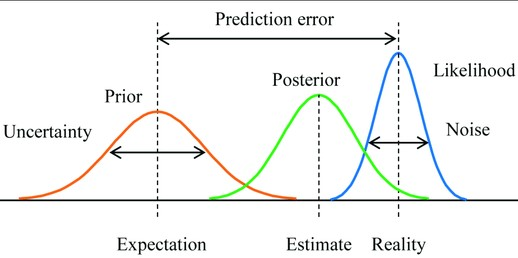
\includegraphics[width=\textwidth]{images/etat_art/bayesian_figure.jpg}
    \end{center}
    \end{figure} 
  \end{minipage}	
\end{frame}

\begin{frame}
  \frametitle{Inférence bayésienne}
  \begin{minipage}{\textwidth}
    \begin{figure}[H]
    \begin{center}
      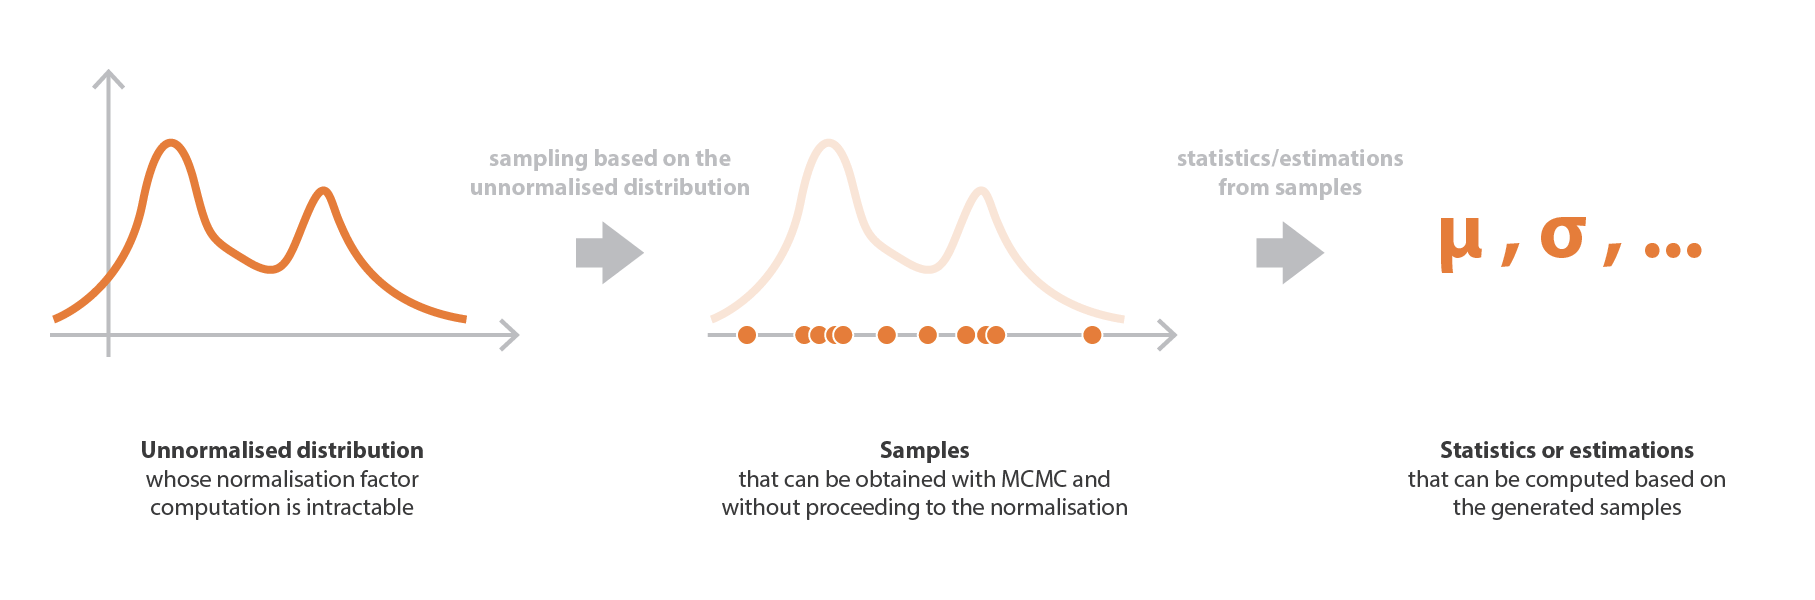
\includegraphics[width=\textwidth]{images/etat_art/mcmc_illustration.png}
    \end{center}
    \end{figure} 
  \end{minipage}	
\end{frame}


\section{CONTRIBUTIONS}

\subsection{Approche proposée}


\begin{frame}
  \justifying 
  \begin{minipage}{\textwidth}
    \begin{center}
      \Huge \textcolor{blueforest}{3. CONTRIBUTIONS} \\
      \vspace{0.5em}
      \huge \hspace{0.5em} Approche proposée
    \end{center}
  \end{minipage}
\end{frame}


\begin{frame}
  \frametitle{Approche proposée}
  \justifying 
  \begin{minipage}{\textwidth}
  \begin{figure}[H]
      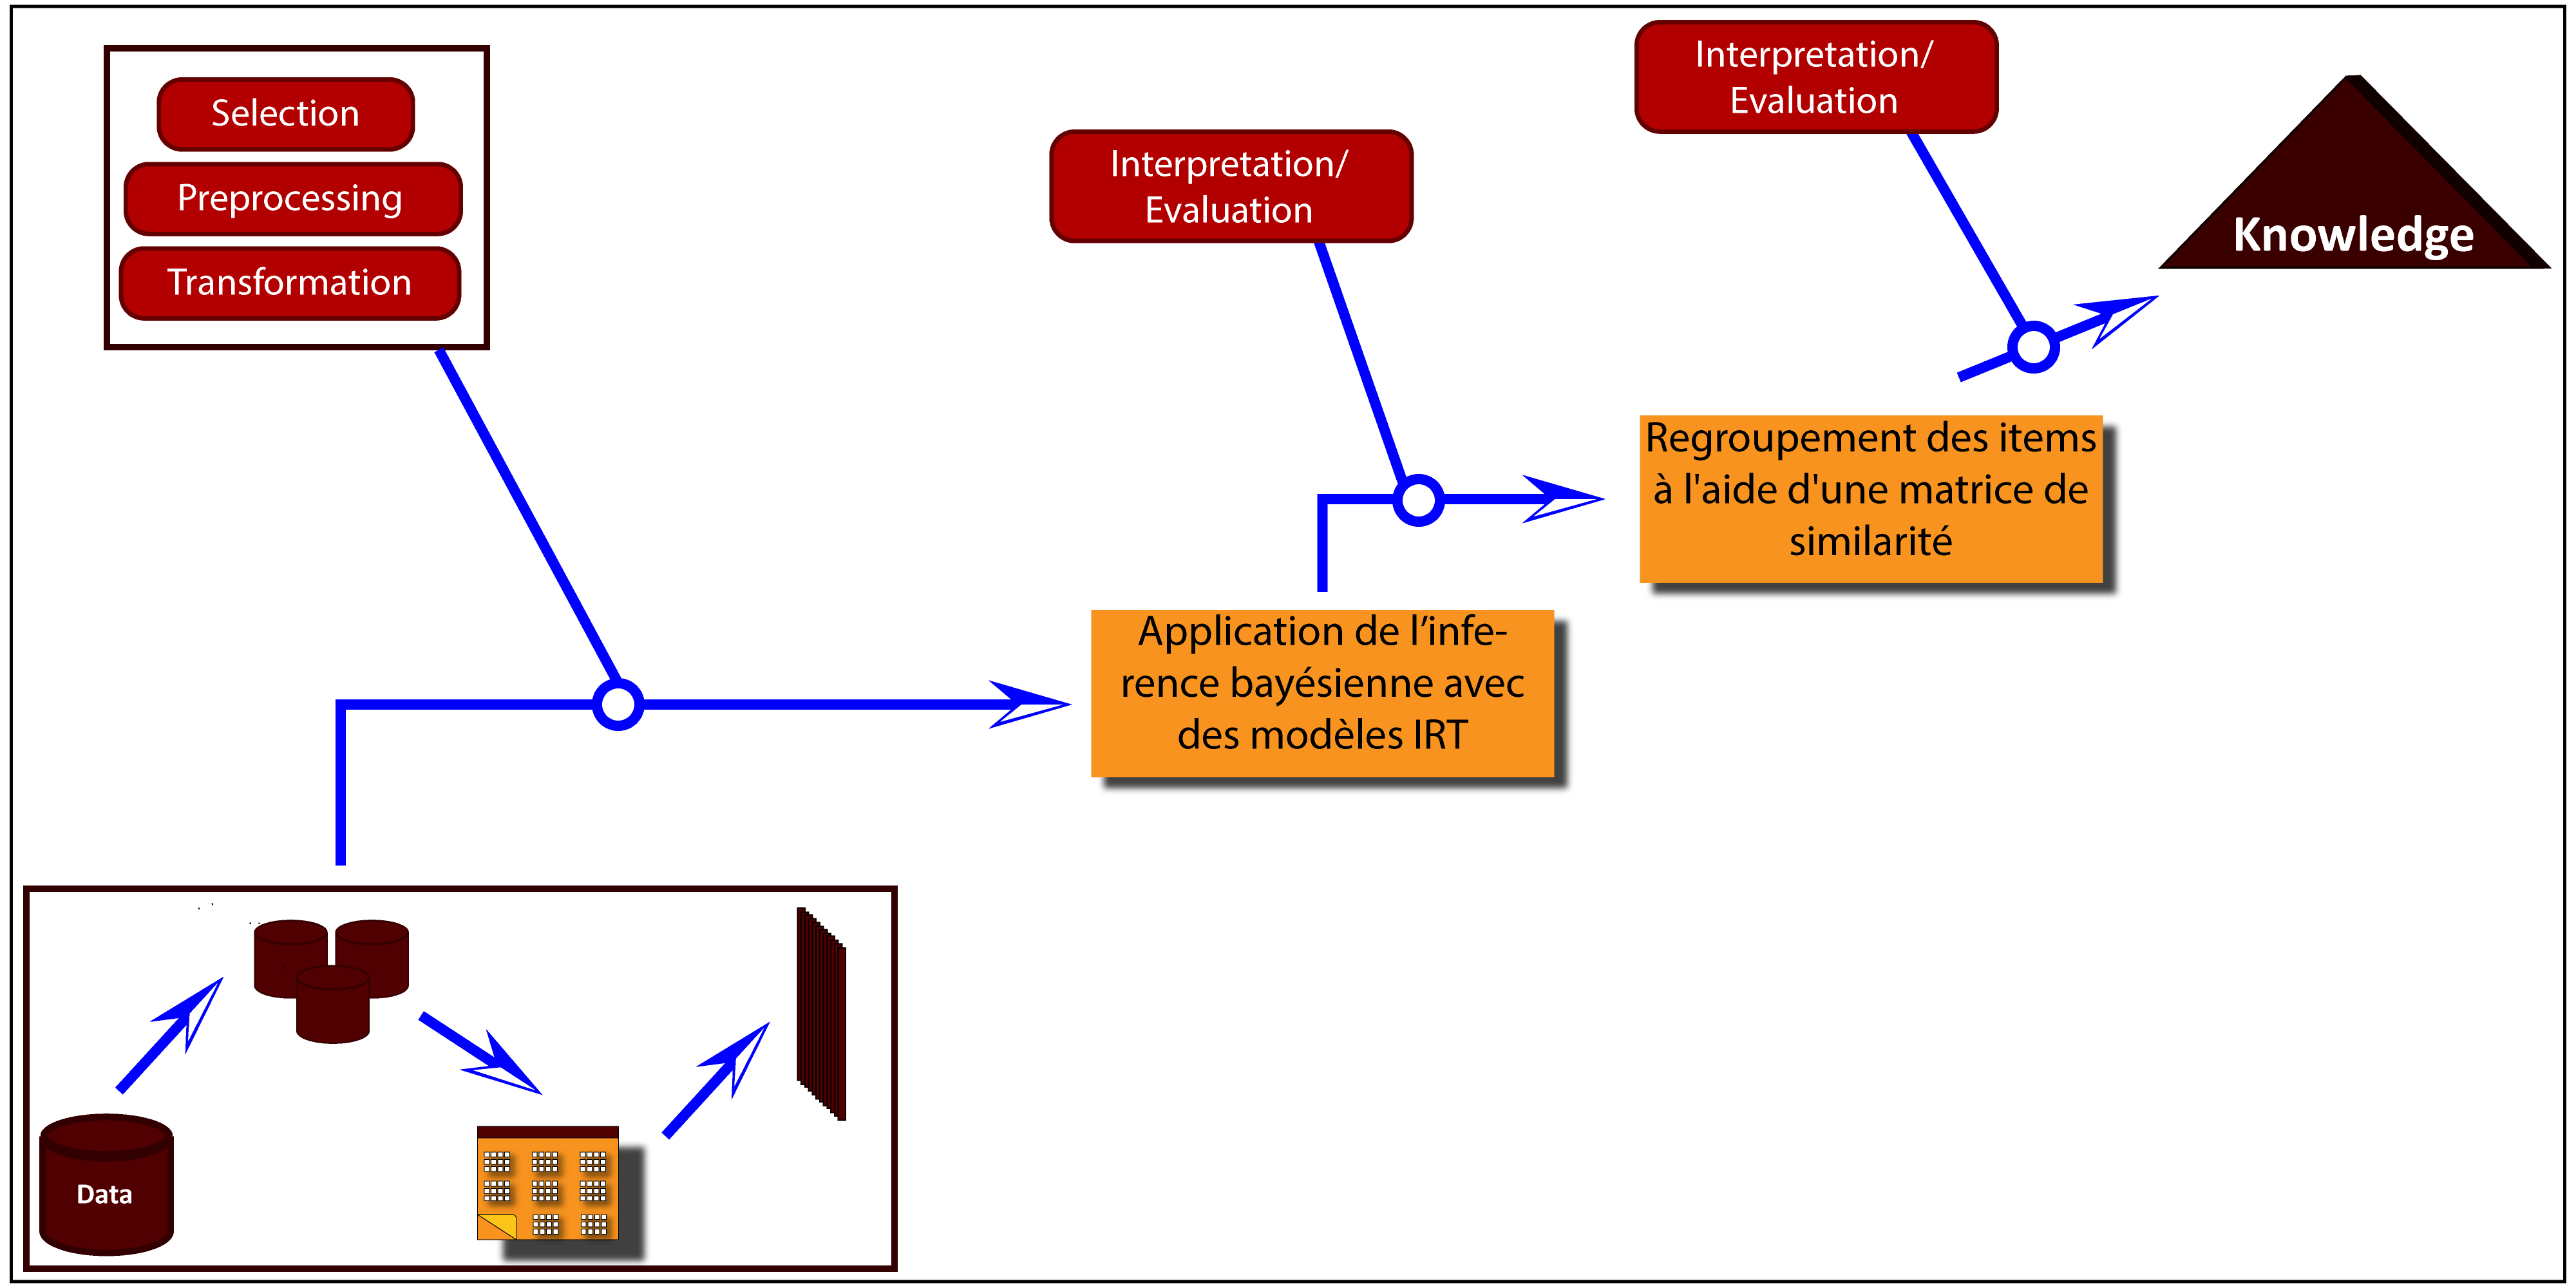
\includegraphics[height=6cm]{images/contribution/aproche.png}
  \end{figure}
  \end{minipage}
\end{frame}


\subsection{Application de l'inférence bayésienne avec des modèles IRT}

\begin{frame}
  \justifying 
  \begin{minipage}{\textwidth}
    \begin{center}
      \huge Application de l'inférence bayésienne avec des modèles IRT
    \end{center}
  \end{minipage}
\end{frame}


\begin{frame}[fragile,plain]{Code}
  \frametitle{Approche proposée}
  \framesubtitle{Application de l'inférence bayésienne avec des modèles IRT}
  \begin{minipage}{0.3\textwidth}
    \begin{figure}[t]
      \begin{center}
        
\includegraphics[scale=0.3]{images/contribution/stan.png}
      \end{center}
    \end{figure}
    \begin{block}{}
      Stan est plate-forme de modélsation statistique et d'inference statistique bayésienne.
    \end{block}
  \end{minipage}
  \begin{minipage}{1mm}
  \hspace{1mm}
  \end{minipage}
  \begin{minipage}{0.5\textwidth}
    \begin{block}{le bloc de données}
      \begin{lstlisting}[language=Stan,basicstyle=\scriptsize,tabsize=1,framesep=0pt,framexleftmargin=0pt,xleftmargin=0pt,xrightmargin=0pt,breakindent=0pt,resetmargins=true]
      functions {
      }
      data {
      }
      parameters {
      }
      transformed parameters {
      }
      model {
      }
      generated quantities {
      }
      \end{lstlisting}
      \end{block}
  \end{minipage}	
\end{frame}

\begin{frame}[fragile,plain]{Code}
  \frametitle{Approche proposée}
  \framesubtitle{Application de l'inférence bayésienne avec des modèles IRT}
  \(\displaystyle \blacksquare \) \textbf{\underline{Spécification et construction des modèles}}
  \begin{minipage}{0.48\textwidth}
    \begin{block}{le bloc de données}
    \begin{lstlisting}[language=Stan,basicstyle=\scriptsize,tabsize=1,framesep=0pt,framexleftmargin=0pt,xleftmargin=0pt,xrightmargin=0pt,breakindent=0pt,resetmargins=true]
    data {
      int<lower=1> N;
      int<lower=1> I;
      int<lower=1> S;
      int<lower=1,upper=I> item[N];
      int<lower=1,upper=S> subject[N];
      int<lower=0,upper=1> grade[N];
    }
    \end{lstlisting}
    \end{block}
  \end{minipage}
  \begin{minipage}{1mm}
  \hspace{1mm}
  \end{minipage}
  \begin{minipage}{0.48\textwidth}
    \begin{block}{Données dans un dictionnaire}
    \begin{lstlisting}[language=Stan,basicstyle=\scriptsize,tabsize=1,framesep=0pt,framexleftmargin=0pt,xleftmargin=0pt,xrightmargin=0pt,breakindent=0pt,resetmargins=true]
      {'I': 1084,
      'N': 809694,
      'S': 574,
      'grade': array([0,...,1]),
      'item': array([563,...,482]),
      'subject': array([72,...,395])}
      \end{lstlisting}
    \end{block}
  \end{minipage}	
\end{frame}


\begin{frame}[fragile]{Code}
  \frametitle{Approche proposée}
  \framesubtitle{Application de l'inférence bayésienne avec des modèles IRT}
  \justifying 
  \(\displaystyle \blacksquare \) \textbf{\underline{Spécification et construction des modèles}}
  \begin{minipage}{\textwidth}
  \begin{block}{le bloc de paramètres}
    \begin{lstlisting}[language=Stan,basicstyle=\scriptsize,framesep=4.5mm,framexleftmargin=2.5mm,tabsize=2]
    parameters {
    real ability[S];             //  alpha: ability of student
    real difficulty[I];          //  beta: difficulty of question
    real delta;                   // mean student ability
    // end for Rasch model
    vector<lower=0>[I] discrimination;      // discrimination of question
    // end for 2PL
    vector<lower=0,upper=1>[I] guessing;    //
    // end for 3PL
    }
    \end{lstlisting}
  \end{block}
  \end{minipage}
\end{frame}

\begin{frame}[fragile]{Code}
  \frametitle{Approche proposée}
  \framesubtitle{Application de l'inférence bayésienne avec des modèles IRT}
  \justifying 
  \(\displaystyle \blacksquare \) \textbf{\underline{Spécification et construction des modèles}}
  \begin{minipage}{\textwidth}
  \begin{block}{le bloc modèle (modèle de Rasch)}
    \begin{lstlisting}[language=Stan,basicstyle=\scriptsize,framesep=4.5mm,framexleftmargin=2.5mm,tabsize=2]
      model {
        ability ~ normal(0,1);   // prior      
        difficulty ~ normal(0,1); // prior   
        delta ~ normal(0.75,1);  // prior 
        for(n in 1:N)
          grade[n] ~ bernoulli_logit(ability[subject[n]] - difficulty[item[n]] + delta);
      }
    \end{lstlisting}
  \end{block}
  \end{minipage}
\end{frame}

\begin{frame}[fragile,plain]{Code}
  \frametitle{Approche proposée}
  \framesubtitle{Application de l'inférence bayésienne avec des modèles IRT}
  \(\displaystyle \blacksquare \) \textbf{\underline{Spécification et construction des modèles}}
  \begin{minipage}{0.48\textwidth}
    \begin{block}{le bloc de données}
      \begin{lstlisting}[language=Stan,basicstyle=\scriptsize,framesep=4.5mm,framexleftmargin=2.5mm,tabsize=2]
        model {
          for(n in 1:N)
            grade[n] ~ bernoulli_logit(ability[subject[n]] - difficulty[item[n]] + delta);
        }
      \end{lstlisting}
    \end{block}
  \end{minipage}
  \begin{minipage}{1mm}
  \hspace{1mm}
  \end{minipage}
  \begin{minipage}{0.48\textwidth}
    \begin{block}{Logit}
      \begin{equation}
        inv\_logit(x) = \frac{\exp(x)}{1+ \exp(x)}
      \end{equation}
    \end{block}
  \end{minipage}

  \begin{minipage}{\textwidth}
    \begin{block}{La fonction logistique du modèle de Rasch}
      \begin{equation}
        P(grade = 1) = \frac{\exp \left[ ability - difficulty + delta  \right]  }{1+ \exp \left[ ability - difficulty + delta \right] }
      \end{equation}
    \end{block}
  \end{minipage}	
\end{frame}

\begin{frame}[fragile]{Code}
  \frametitle{Approche proposée}
  \framesubtitle{Application de l'inférence bayésienne avec des modèles IRT}
  \justifying 
  \(\displaystyle \blacksquare \) \textbf{\underline{Spécification et construction des modèles}}
  \begin{minipage}{\textwidth}
  \begin{block}{bloc modèle (modèle 2PL)}
    \begin{lstlisting}[language=Stan,basicstyle=\scriptsize,framesep=4.5mm,framexleftmargin=2.5mm,tabsize=2]
      model {
        ability ~ normal(0,1);         // prior
        difficulty ~ normal(0,1);   // prior
        discrimination ~ lognormal(0,1);   // prior
        delta ~ normal(0.75,1);     // prior
        grade ~ bernoulli_logit(discrimination[item] .* (ability[subject] - (difficulty[item] + delta)));	
      }
    \end{lstlisting}
  \end{block}
  \end{minipage}
\end{frame}

\begin{frame}[fragile]{Code}
  \frametitle{Approche proposée}
  \framesubtitle{Application de l'inférence bayésienne avec des modèles IRT}
  \justifying 
  \(\displaystyle \blacksquare \) \textbf{\underline{Spécification et construction des modèles}}
  \begin{minipage}{\textwidth}
  \begin{block}{bloc modèle (modèle 3PL)}
    \begin{lstlisting}[language=Stan,basicstyle=\scriptsize,framesep=4.5mm,framexleftmargin=2.5mm,tabsize=2]
      model {
        ability ~ normal(0,1);         
        difficulty ~ normal(0,1);   
        discrimination ~ lognormal(0,1);
        guessing ~ beta(5,17);
        delta ~ normal(0.75,1);
        grade ~ bernoulli(guessing[item] + ((1-guessing[item]).*(inv_logit(discrimination[item] .* (ability[subject] - (difficulty[item] + delta))))));
      }
    \end{lstlisting}
  \end{block}
  \end{minipage}
\end{frame}


\begin{frame}[fragile]{Code}
  \frametitle{Approche proposée}
  \framesubtitle{Application de l'inférence bayésienne avec des modèles IRT}
  \(\displaystyle \blacksquare \) \textbf{\underline{ Inférence }}

  \justifying 
  \begin{minipage}{\textwidth}
  \begin{block}{Compilation}
    \begin{lstlisting}[language=Stan,basicstyle=\small,framesep=4.5mm,framexleftmargin=2.5mm,tabsize=2]
      posteriori = stan.build(_1pl_model,data=train_data,random_seed=2021)
    \end{lstlisting}
  \end{block}
  \begin{block}{\'Echantillonnage}
    \begin{lstlisting}[language=Stan,basicstyle=\small,framesep=4.5mm,framexleftmargin=2.5mm,tabsize=2]
      fit = posteriori.sample(num_chains=4, num_samples=2000,num_warmup=1000,num_thin=1)
    \end{lstlisting}
  \end{block}
  \end{minipage}
\end{frame}

\begin{frame}
  \frametitle{Approche proposée}
  \framesubtitle{Application de l'inférence bayésienne avec des modèles IRT}
  \(\displaystyle \blacksquare \) \textbf{\underline{ Diagnostic de convergence }} \\
  \justifying 
  \begin{minipage}{\textwidth}
  \begin{block}{Rhat}
    Rhat fait référence à la statistique de réduction d'échelle potentielle, également connue sous le nom de statistique de Gelman-Rubin.
  \end{block}
  \end{minipage}
 
\end{frame}

\begin{frame}
  \justifying 
  \begin{minipage}{\textwidth}
    \begin{figure}[H]
      \begin{center}
        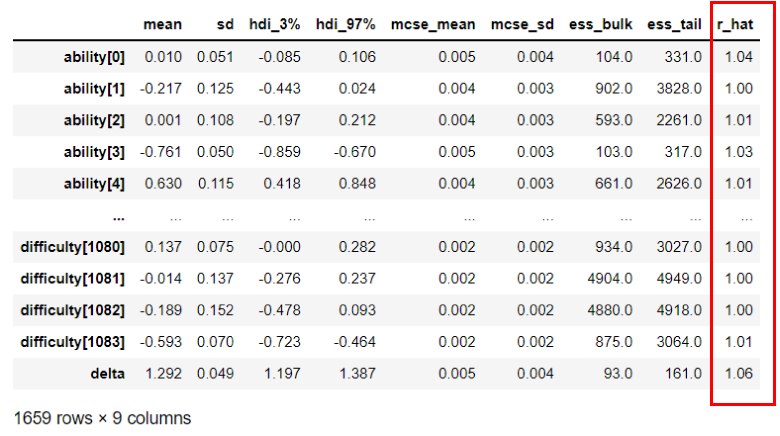
\includegraphics[width=\textwidth]{images/contribution/output_of_rhat.png}
      \end{center}
    \end{figure}
  \end{minipage}
\end{frame}


\subsection{Résultats des modèles IRT}

\begin{frame}
  \justifying 
  \begin{minipage}{\textwidth}
    \begin{center}
      \huge Résultats des modèles IRT
    \end{center}
  \end{minipage}
\end{frame}

\begin{frame}
  \frametitle{Résultats des modèles IRT}
  \justifying 
  \begin{minipage}{\textwidth} 
  \begin{figure}[H]
    \begin{center}
      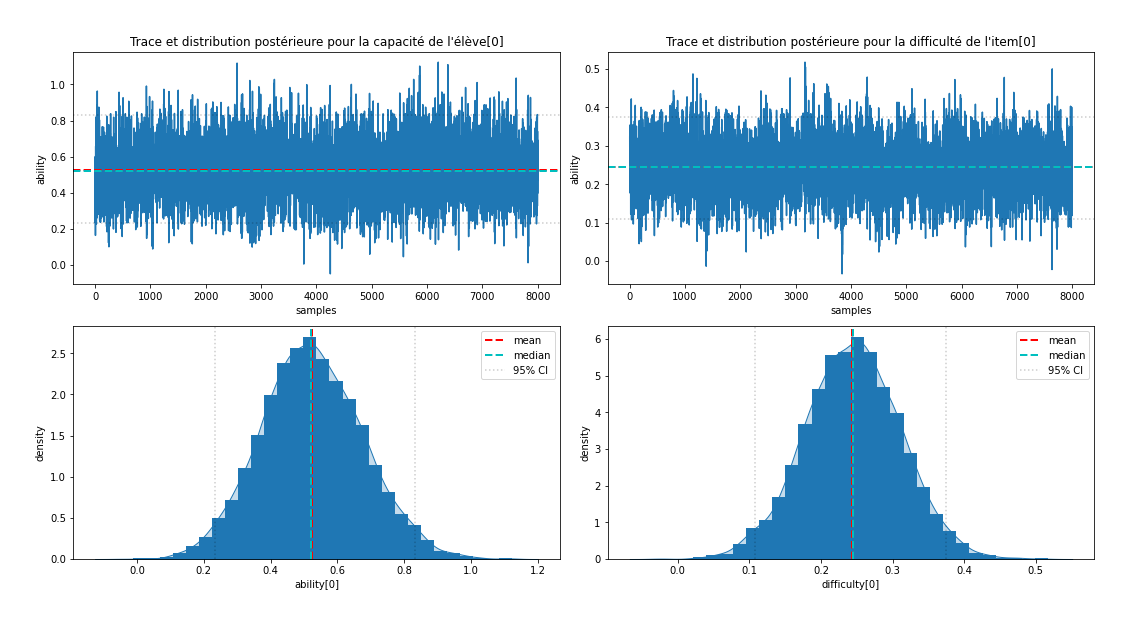
\includegraphics[scale=0.3]{images/contribution/params_posterior_distribution.png}
    \end{center}
  \end{figure}
  \end{minipage}
\end{frame}

\begin{frame}
  \frametitle{Résultats des modèles IRT}
  \justifying 
  \begin{minipage}{\textwidth}
    \begin{figure}[H]
      \begin{center}
        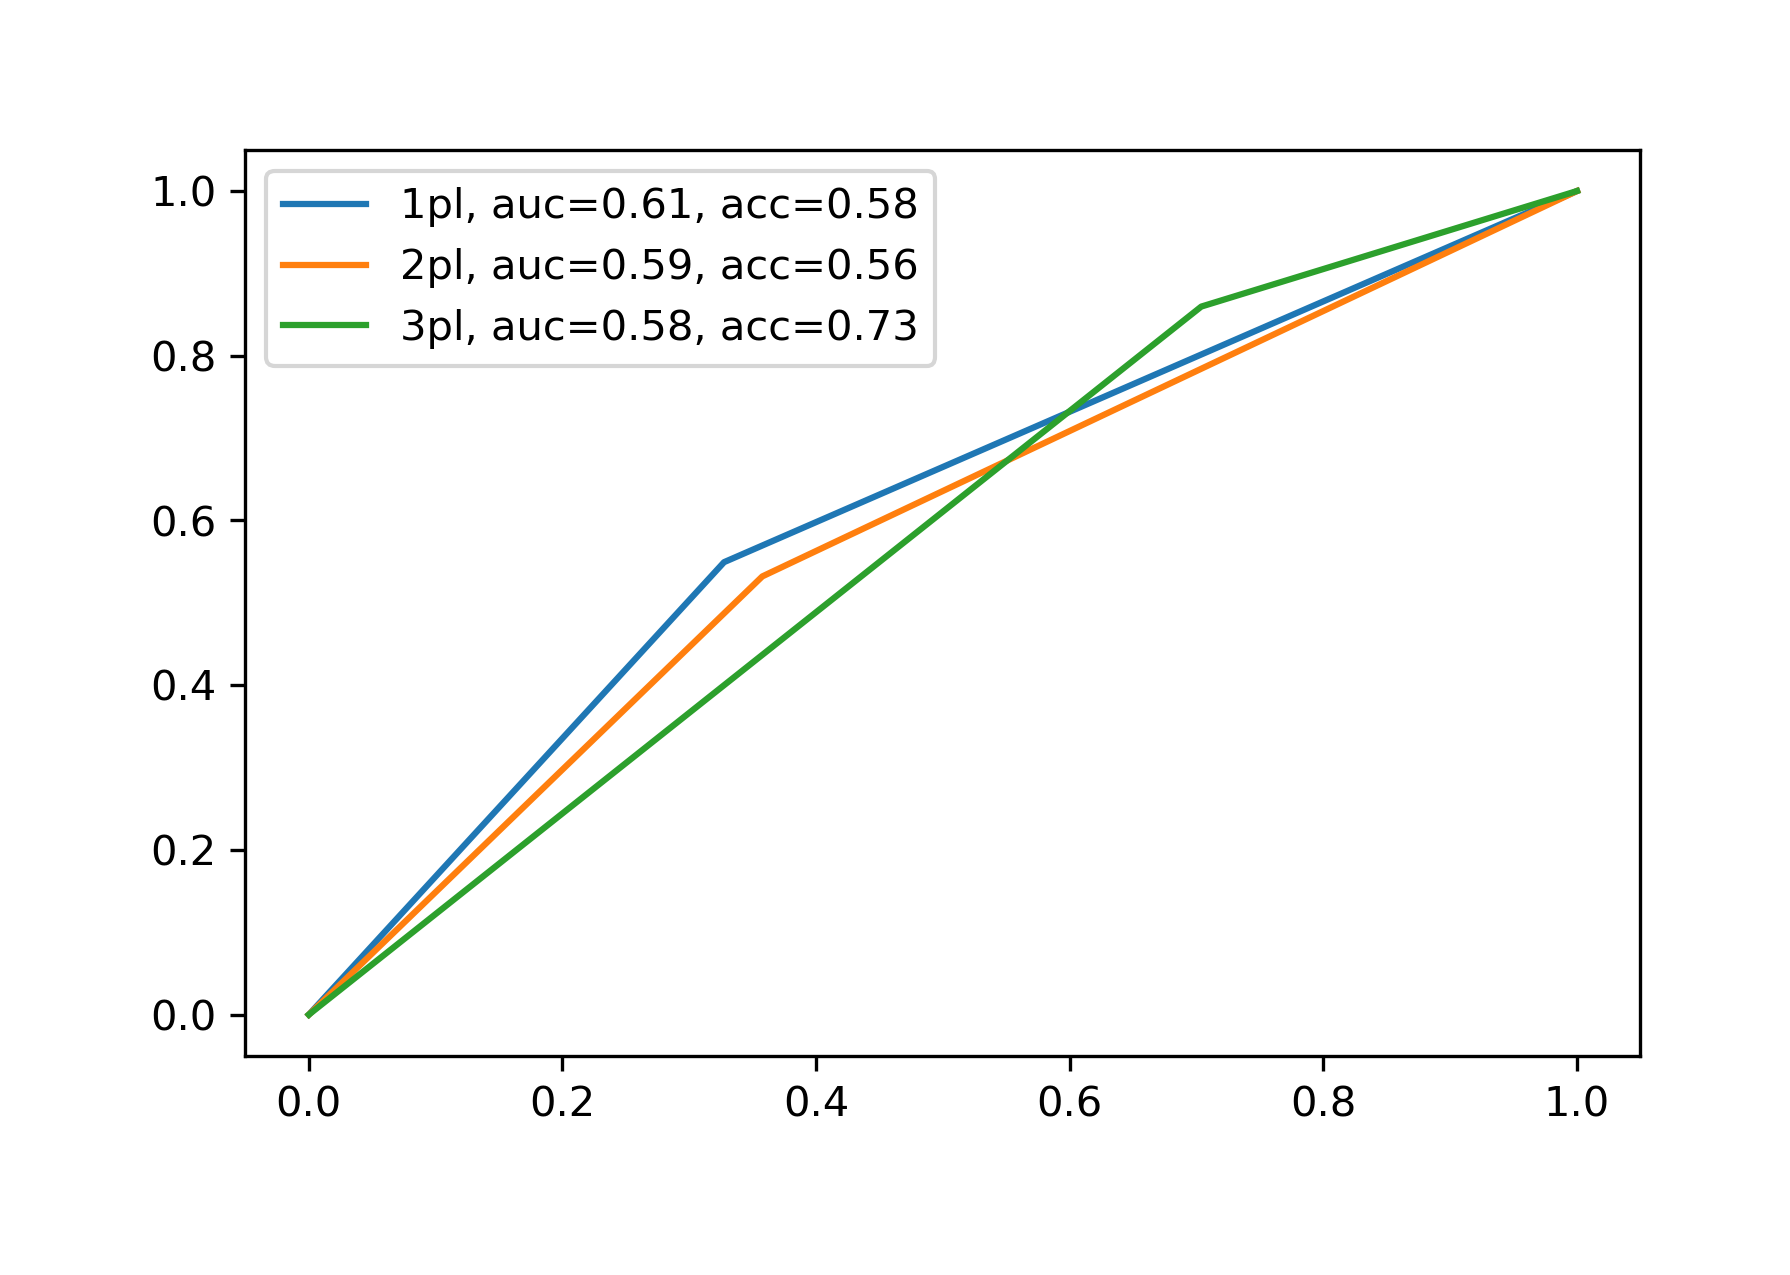
\includegraphics[scale=0.6]{images/contribution/roc_auc.png}
      \end{center}
    \end{figure}
  \end{minipage}
\end{frame}

\begin{frame}
  \frametitle{Résultats des modèles IRT}
  \justifying 
  \begin{minipage}{\textwidth}
    \begin{figure}[H]
      \begin{center}
        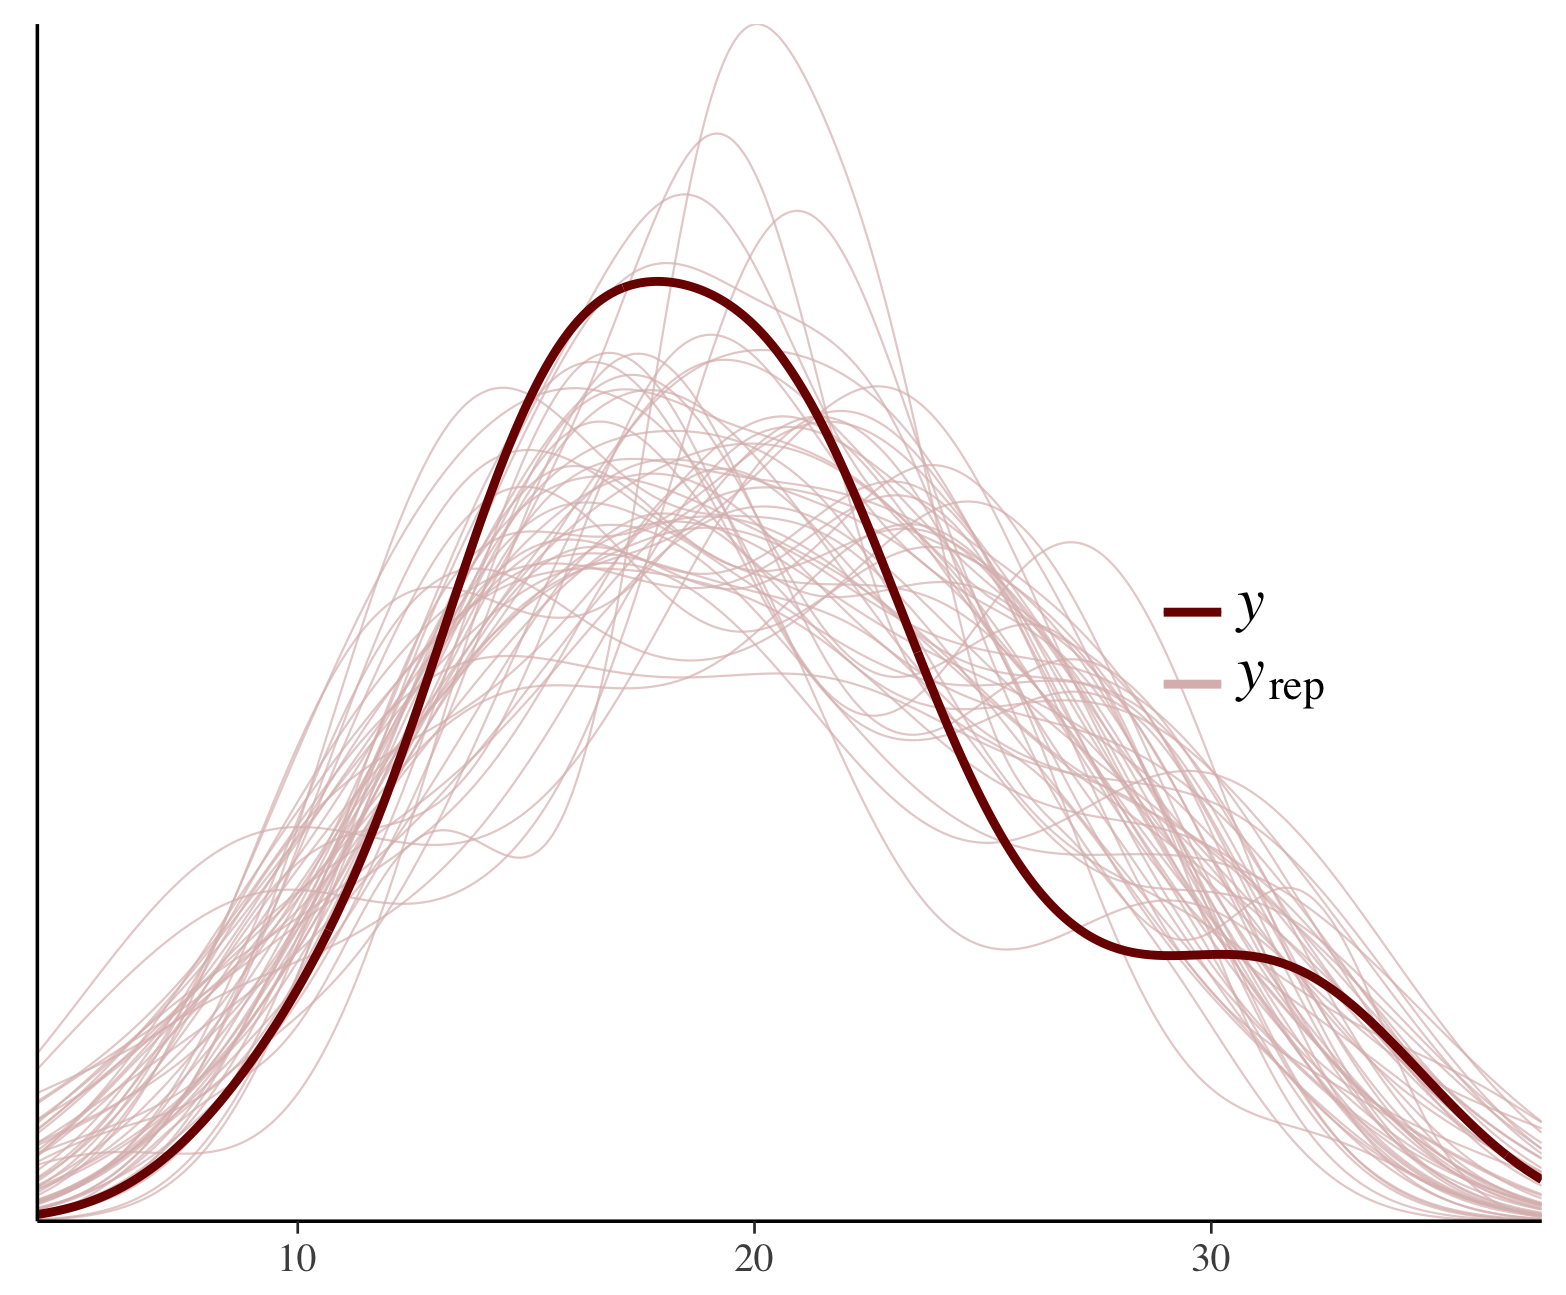
\includegraphics[scale=0.11]{images/etat_art/ppc.png}
      \end{center}
    \end{figure}
  \end{minipage}
\end{frame}

\begin{frame}
  \frametitle{Résultats des modèles IRT}
  \justifying
  \begin{minipage}{\textwidth}
    \begin{figure}[H]
      \begin{center}
        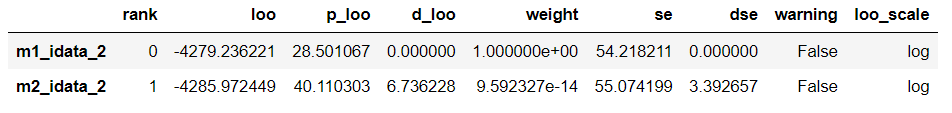
\includegraphics[scale=0.6]{images/etat_art/model_selection.png}
      \end{center}
    \end{figure}
  \end{minipage}
\end{frame}

\subsection{Regroupement des items à l’aide de la matrice de similarité}

\begin{frame}
  \justifying 
  \begin{minipage}{\textwidth}
    \begin{center}
      \huge Regroupement des items à l’aide de la matrice de similarité
    \end{center}
  \end{minipage}
\end{frame}

\begin{frame}
  \justifying 
  \begin{minipage}{\textwidth}
    \begin{figure}[H]
      \begin{center}
        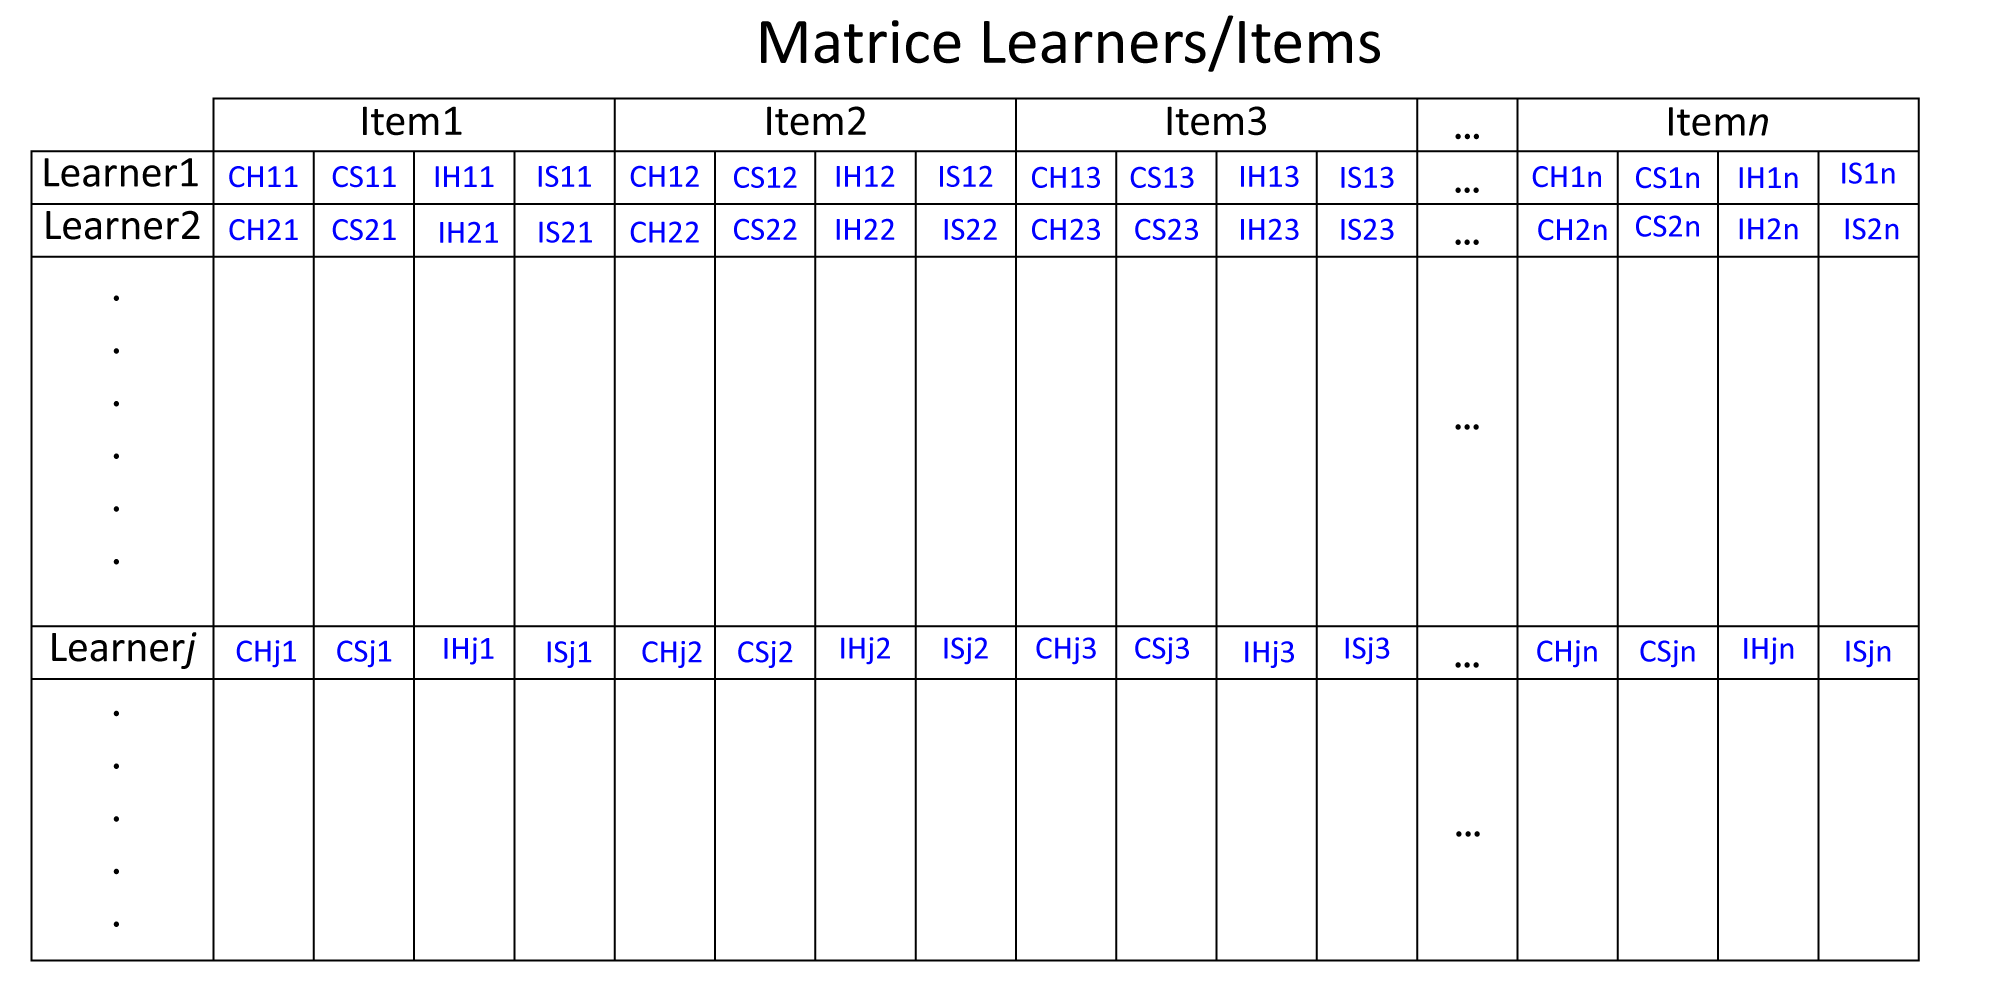
\includegraphics[scale=0.18]{images/contribution/matrice_learners-items.png}
      \end{center}
    \end{figure}
  \end{minipage}
\end{frame}

\begin{frame}
  \frametitle{Approche proposée}
  \framesubtitle{Regroupement des items à l’aide de la matrice de similarité}
  \justifying 
  \begin{minipage}{\textwidth}
    \begin{figure}[H]
      \begin{center}
        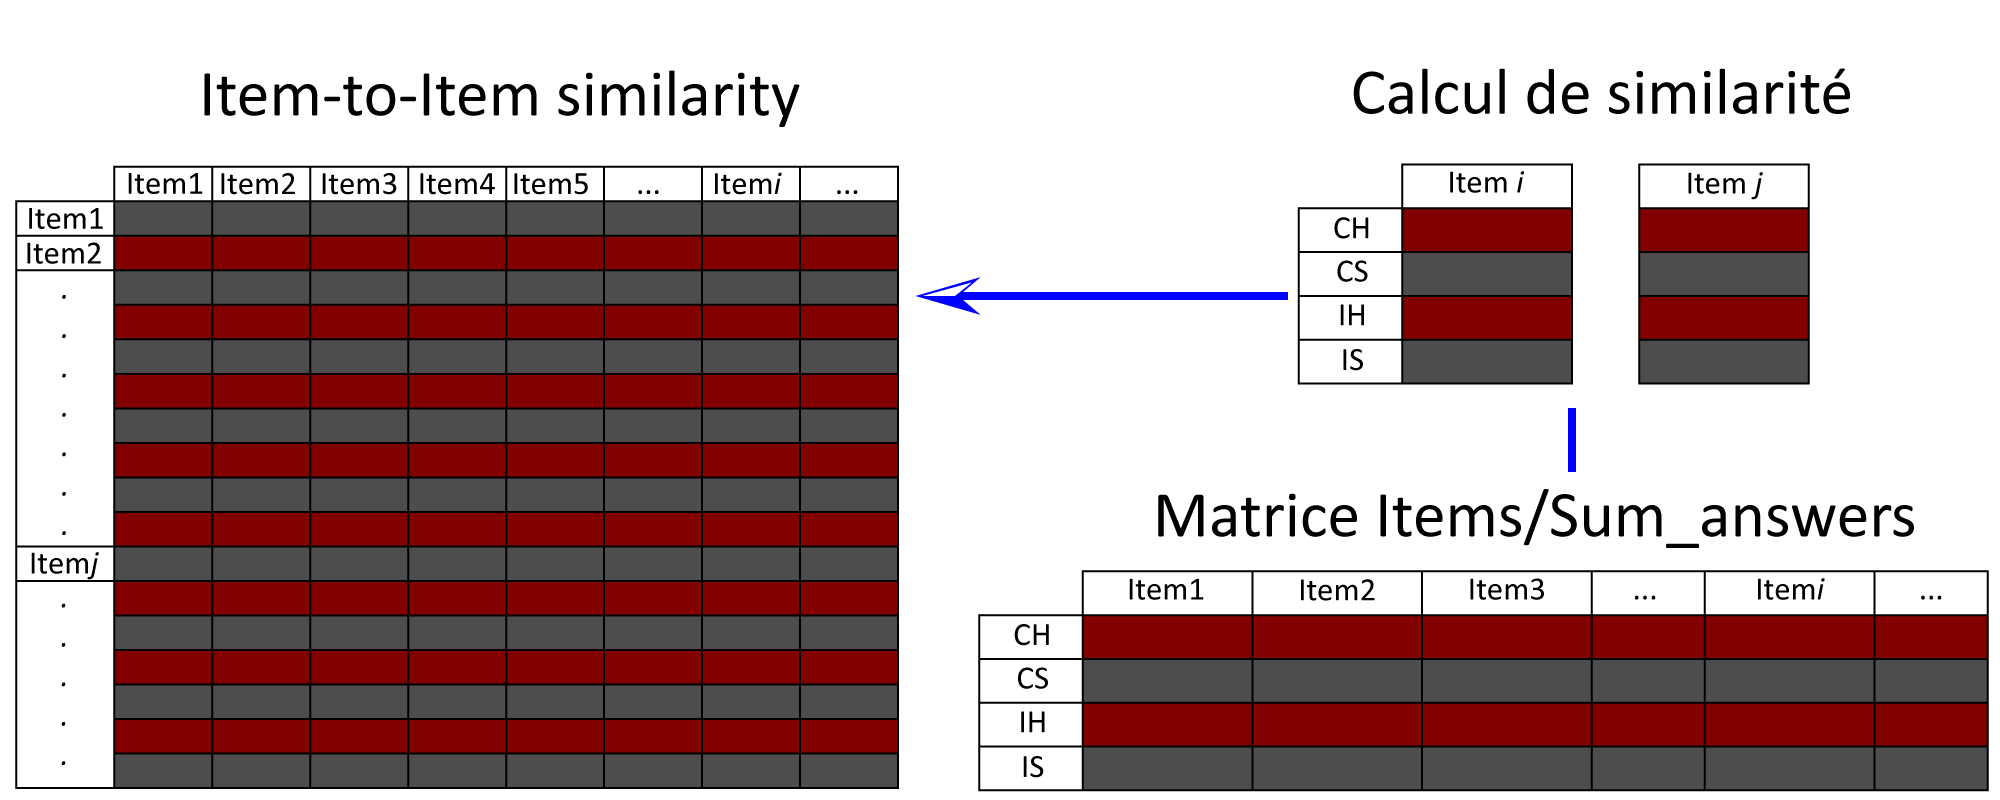
\includegraphics[scale=0.21]{images/contribution/similarity_compute.png}
      \end{center}
    \end{figure}
  \end{minipage}
\end{frame}

\begin{frame}
  \frametitle{Approche proposée}
  \framesubtitle{Regroupement des items à l’aide de la matrice de similarité}
  \(\displaystyle \blacksquare \) \textbf{\underline{Les méthodes de clustering utilisées :}} \\
  \justifying 
  \begin{minipage}{\textwidth}
    \vspace{2em}
  \hspace{3em} \textcolor{blue}{ 1 : \textbf{\underline{ K-means clustering}}}
  \end{minipage}
\end{frame}

\begin{frame}
  \justifying
  \begin{minipage}{\textwidth}
    \begin{figure}[H]
      \begin{center}
        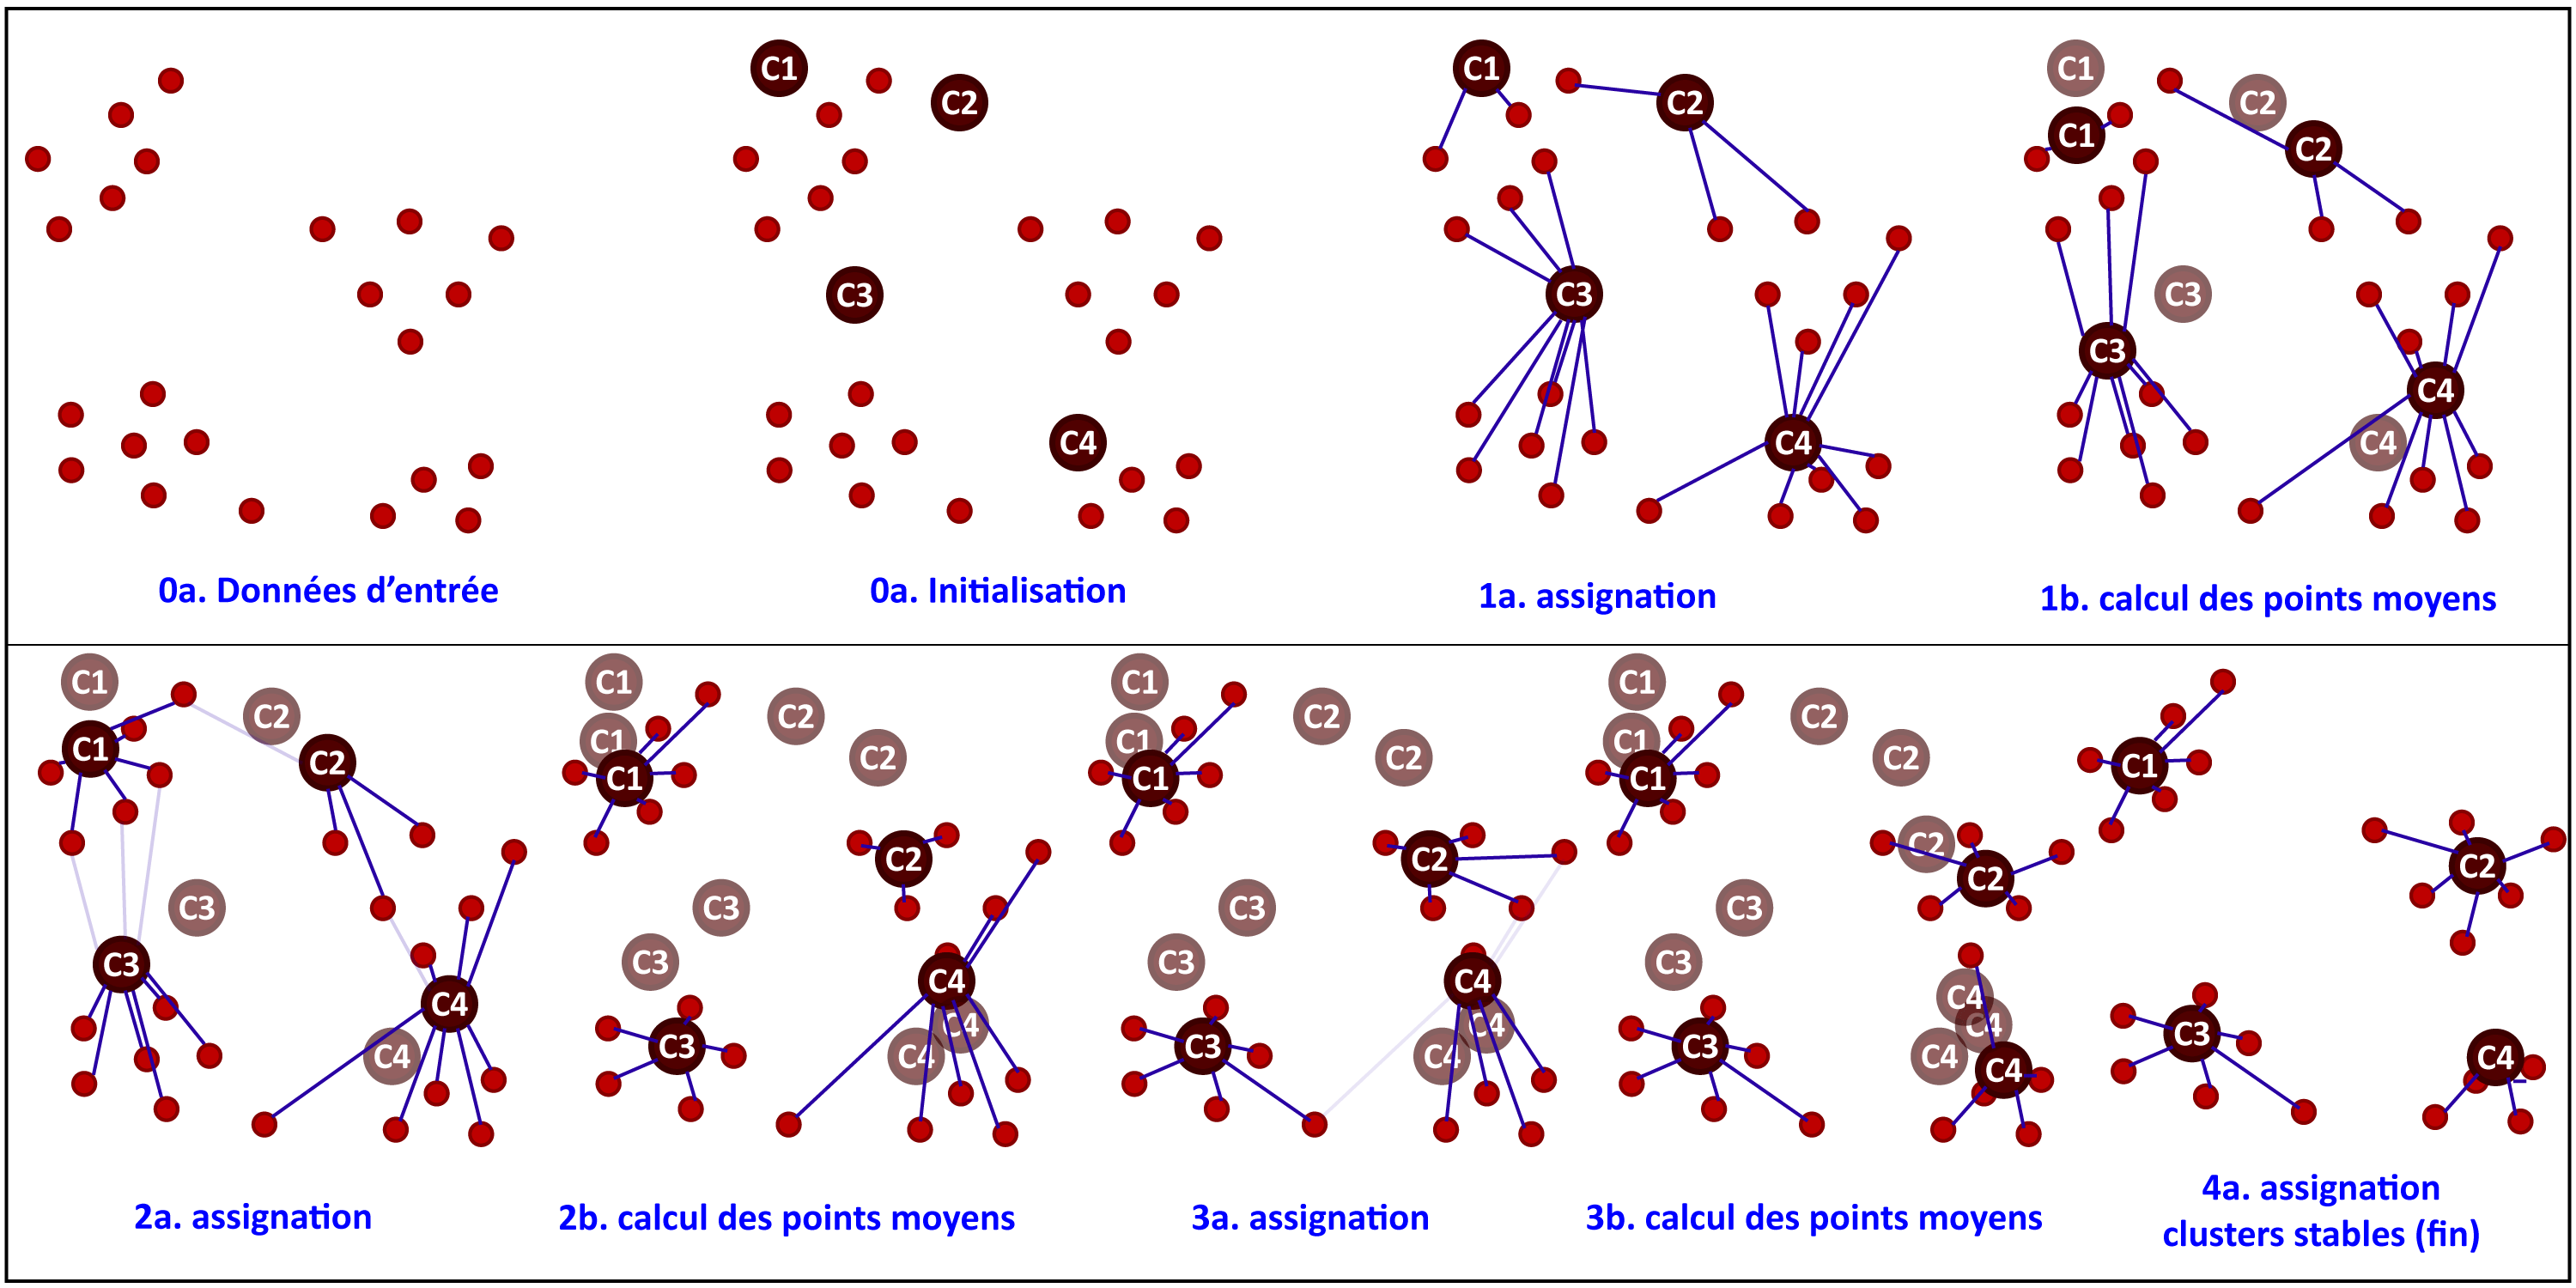
\includegraphics[width=\textwidth]{images/contribution/kmeans_steps.png}
      \end{center}
      \label{kmeans_steps}
    \end{figure}
  \end{minipage}
\end{frame}

\begin{frame}
  \frametitle{Approche proposée}
  \framesubtitle{Regroupement des items à l’aide de la matrice de similarité}
  \(\displaystyle \blacksquare \) \textbf{\underline{Les méthodes de clustering utilisées :}} \\
  \justifying 
  \begin{minipage}{\textwidth}
    \vspace{2em}
  \hspace{3em} \textcolor{blue}{ 2 :\textbf{\underline{ Clustering hiérarchique agglomératif}}}
  \end{minipage}
\end{frame}

\begin{frame}
  \justifying
  \begin{minipage}{\textwidth}
    \begin{figure}[H]
      \centering
        \subfloat{{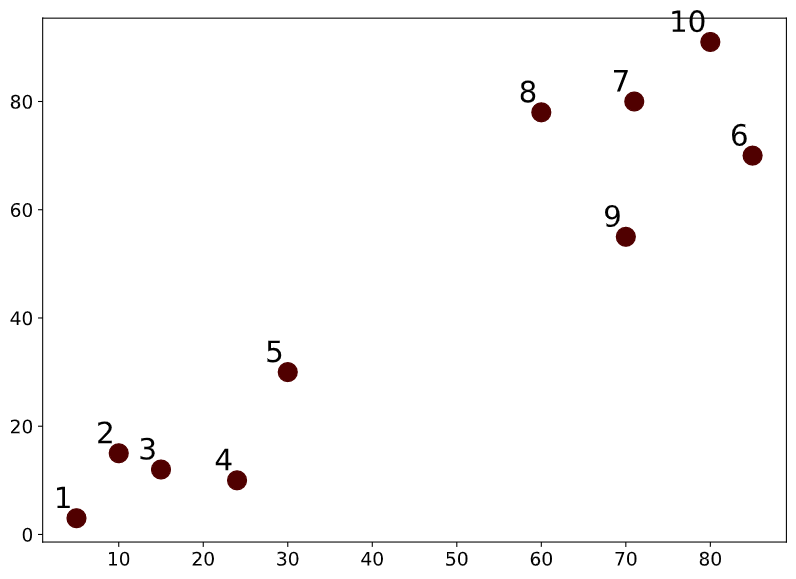
\includegraphics[width=5cm]{images/contribution/agglo_clustering.png} }}%
        \qquad
        \subfloat{{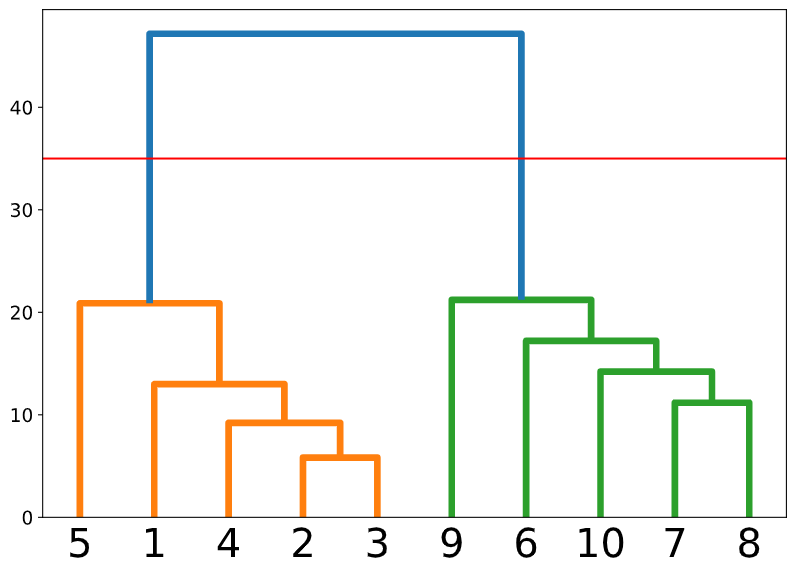
\includegraphics[width=6cm]{images/contribution/dendrogram.png} }}%
        %\caption{Dendrogramme}%
    \end{figure}
  \end{minipage}
\end{frame}

\begin{frame}
  \frametitle{Approche proposée}
  \framesubtitle{Regroupement des items à l’aide de la matrice de similarité}
  \(\displaystyle \blacksquare \) \textbf{\underline{Les méthodes de clustering utilisées :}} \\
  \justifying 
  \begin{minipage}{\textwidth}
    \vspace{2em}
  \hspace{3em} \textcolor{blue}{ 3 :\textbf{\underline{ Fuzzy clustering}}}
  \end{minipage}
\end{frame}

\begin{frame}
  \justifying
  \begin{minipage}{\textwidth}
    \begin{figure}[!h]
      \centering
      \subfloat{{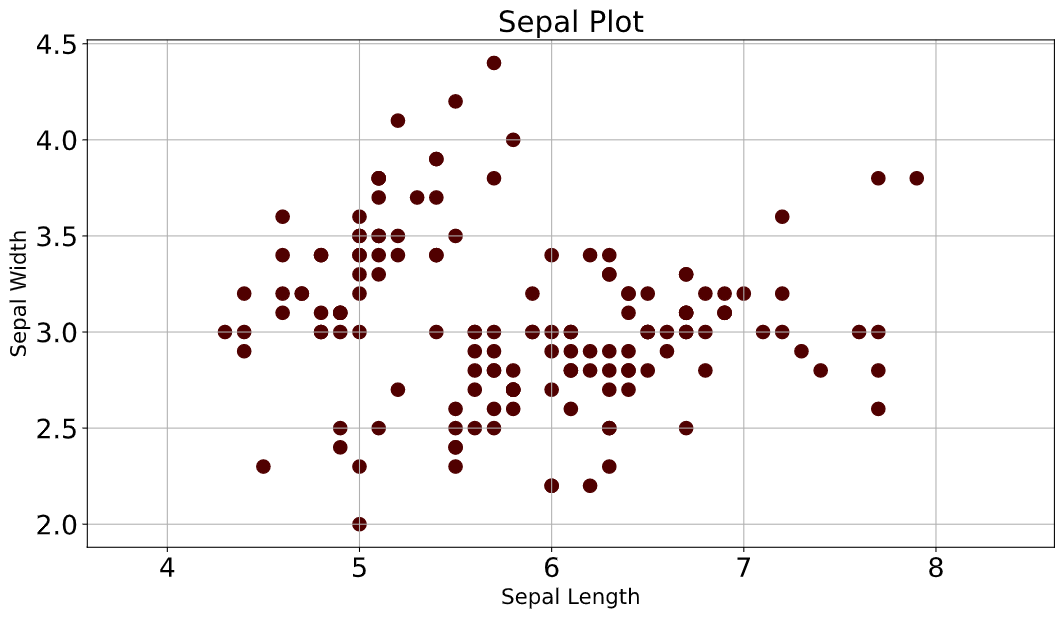
\includegraphics[width=6cm]{images/contribution/data_for_fuzzy.png} }}%
      \qquad
      \subfloat{{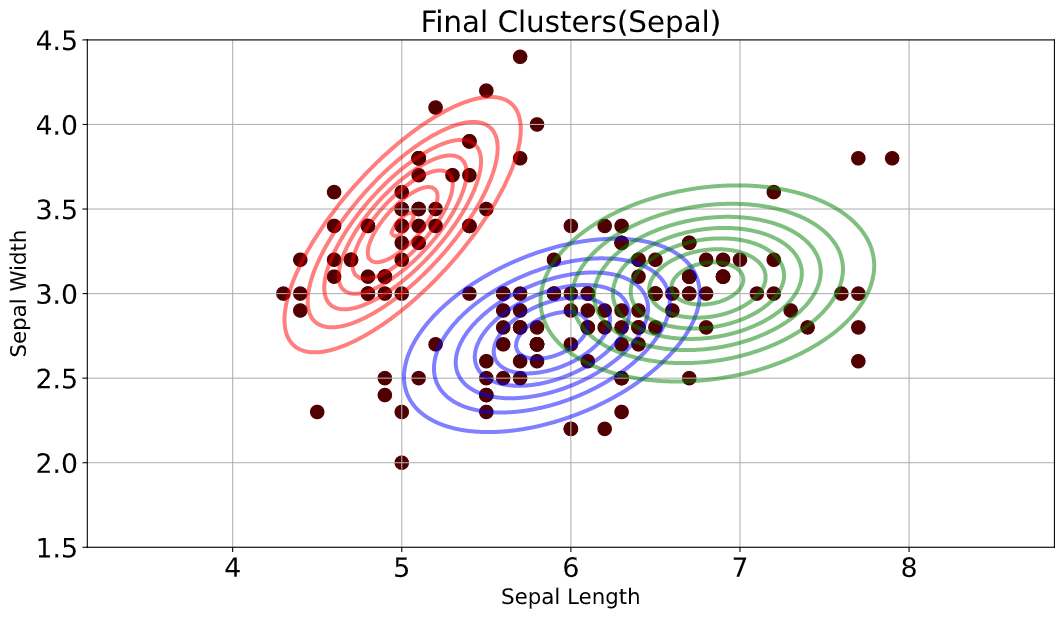
\includegraphics[width=7cm]{images/contribution/fuzzyExemple.png} }}%
      %\caption{Dendrogramme}%
    \end{figure}
  \end{minipage}
\end{frame}


\subsection{Résultats des méthodes de clustering}

\begin{frame}
  \justifying 
  \begin{minipage}{\textwidth}
    \begin{center}
      \huge Résultats des méthodes de clustering
    \end{center}
  \end{minipage}
\end{frame}

\begin{frame}
  \(\displaystyle \blacksquare \) \textbf{\underline{Réduction de dimensionnalité avec ACP}} \\
  \vspace{0.5em}
  \justifying
  \begin{minipage}{\textwidth}
    \begin{figure}[H]
      \centering
      \subfloat{{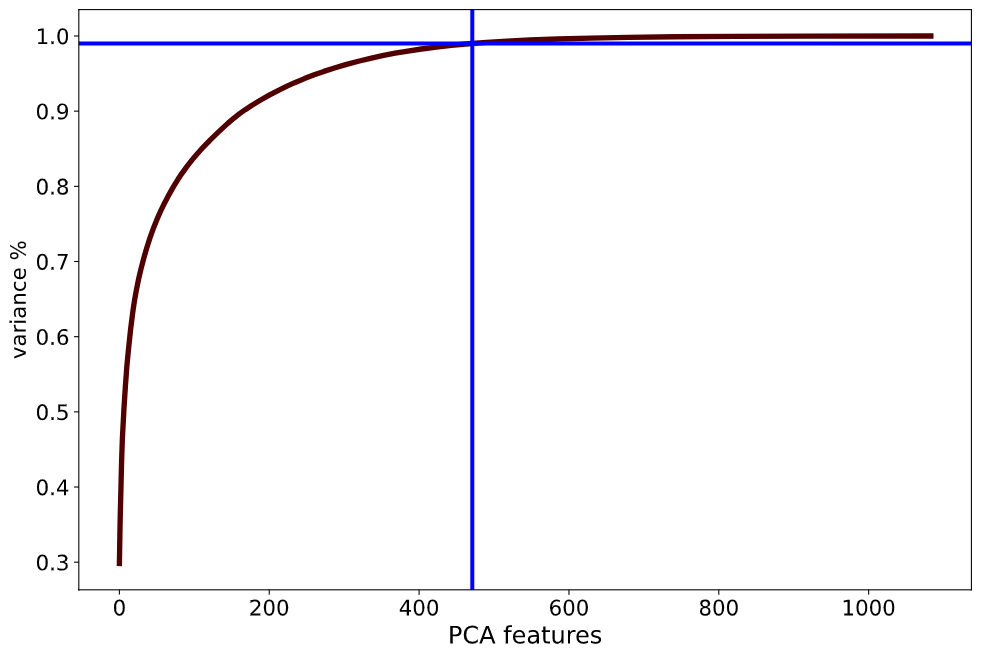
\includegraphics[width=7cm]{images/contribution/pca_variance_ratio1.png}}}%
      \qquad
      \subfloat{{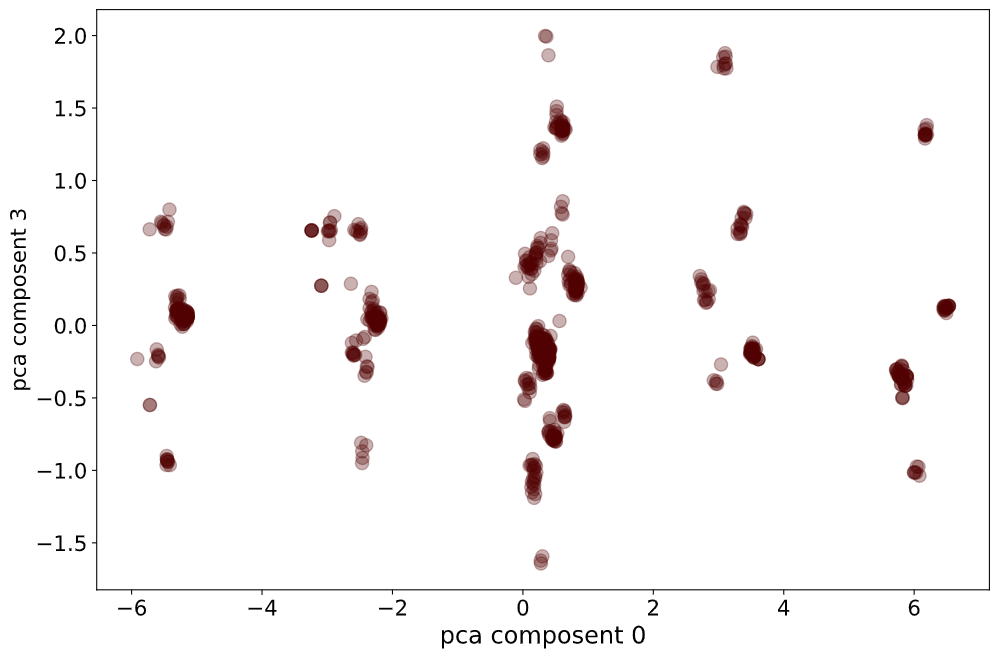
\includegraphics[width=6cm]{images/contribution/pca_features_compress1.png}}}%
      %\caption{Dendrogramme}%
    \end{figure}
  \end{minipage}
\end{frame}

\begin{frame}
  \(\displaystyle \blacksquare \) \textbf{\underline{Clustering hiérarchique agglomératif}} \\
  \justifying 
  \begin{minipage}{\textwidth}
    \begin{figure}[H]
      \begin{center}
        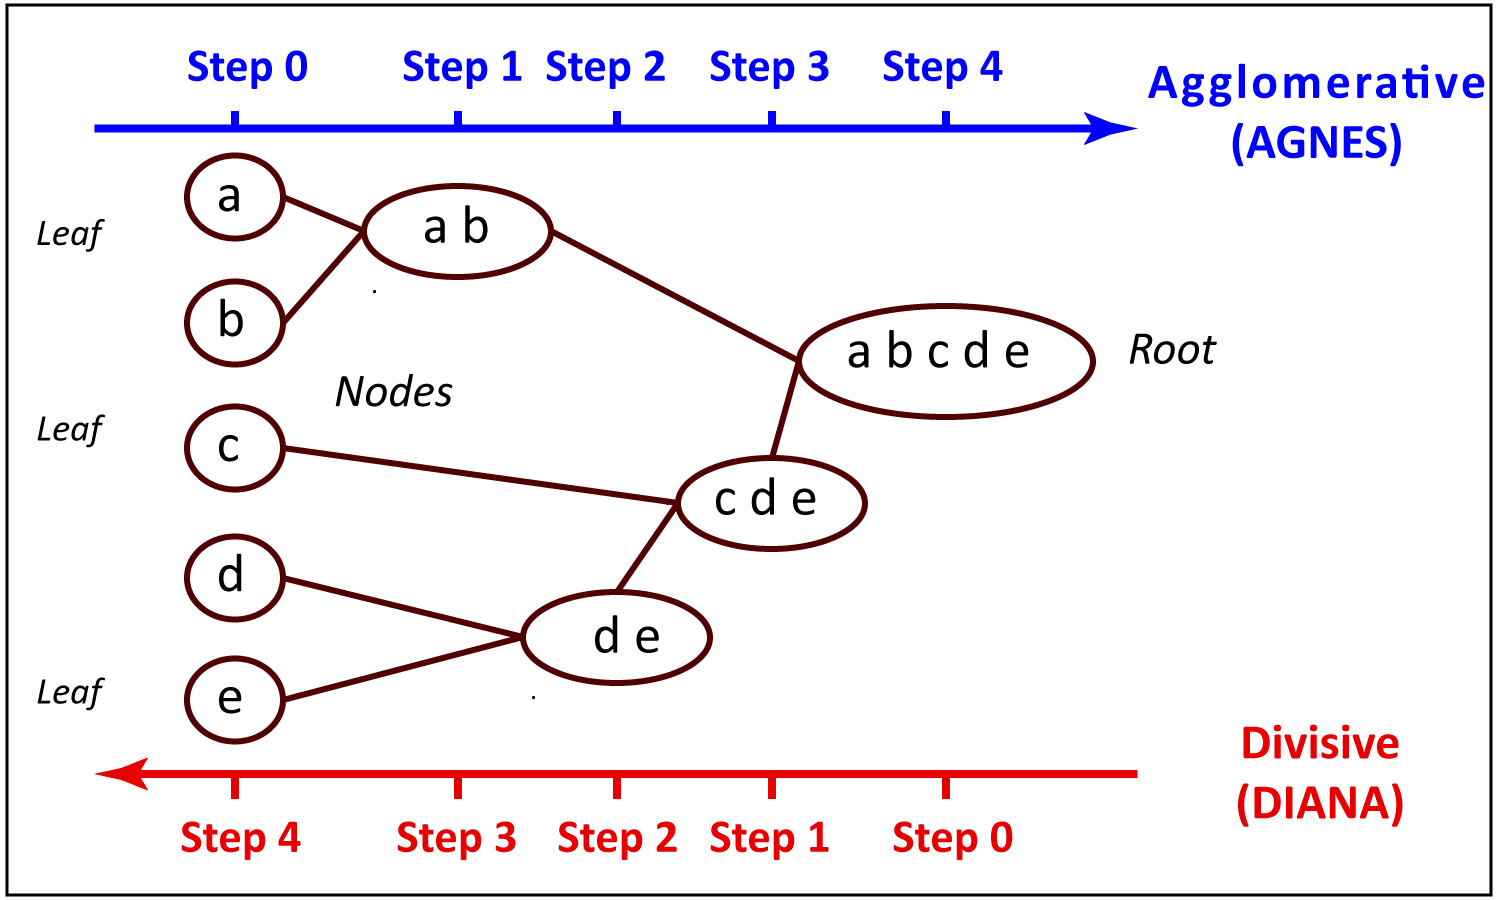
\includegraphics[scale=0.18]{images/contribution/hierarchical_agglo_divisive.png}
      \end{center}
    \end{figure}
  \end{minipage}
\end{frame}

\begin{frame}
  \(\displaystyle \blacksquare \) \textbf{\underline{Clustering hiérarchique agglomératif}} \\
  \justifying
  \begin{minipage}{\textwidth}
    \begin{figure}[H]
      \centering
      \subfloat{{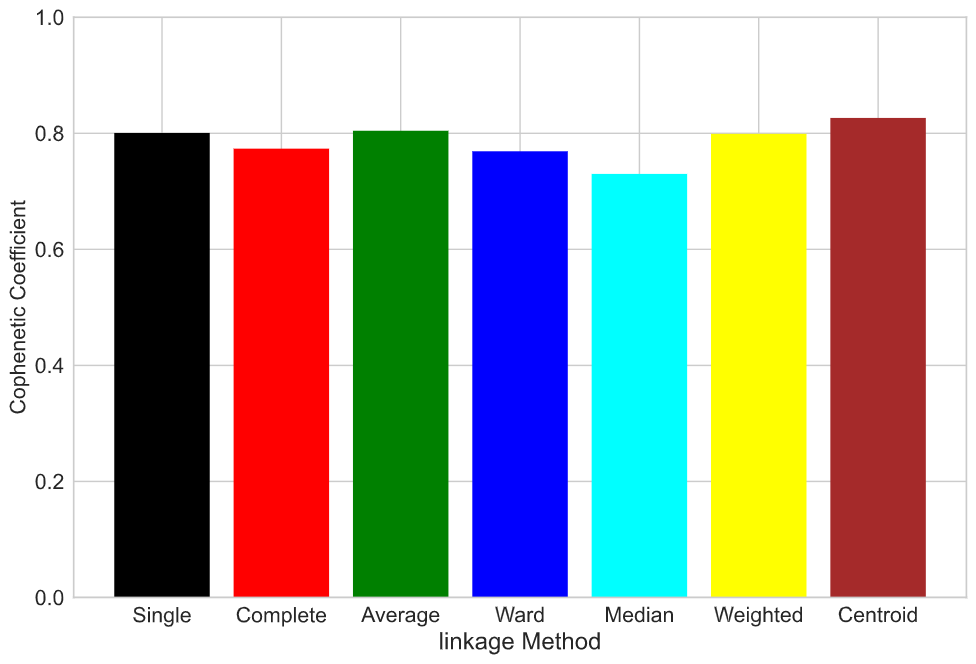
\includegraphics[width=5cm]{images/contribution/linkage_method_score1.png}  }}%
      \qquad
      \subfloat{{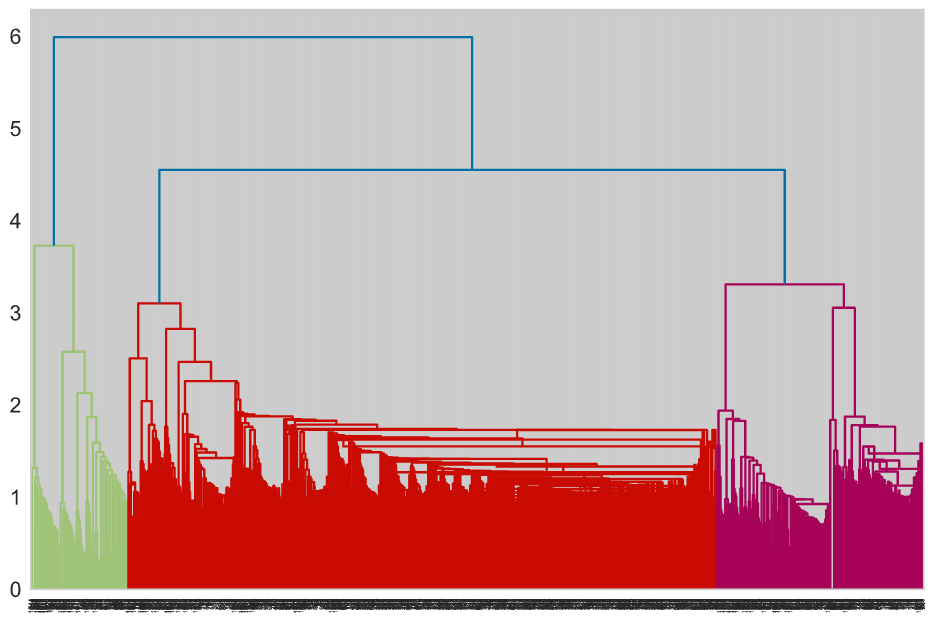
\includegraphics[width=7cm]{images/contribution/dendrogram_of_dataset1.png} } }%
      %\caption{Dendrogramme}%
    \end{figure}
  \end{minipage}
\end{frame}

\begin{frame}
  \justifying
  \begin{minipage}{\textwidth}
    \begin{figure}[H]
      \begin{center}
        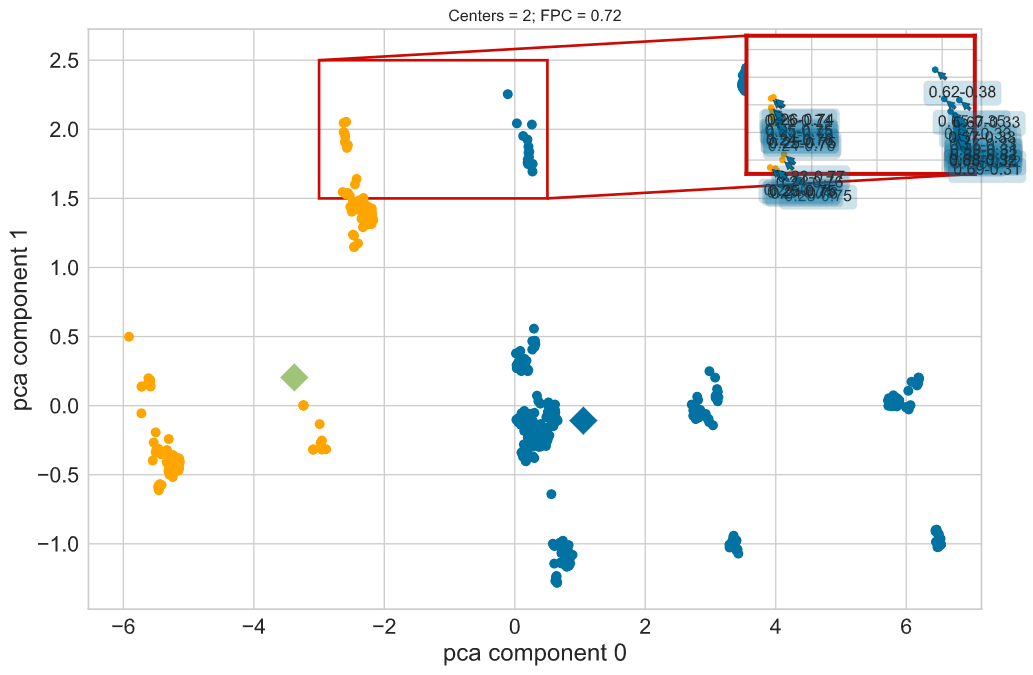
\includegraphics[scale=0.4]{images/contribution/fuzzy_partition_plot1.png}
      \end{center}
    \end{figure}
  \end{minipage}
\end{frame}

\section{CONCLUSION G\'EN\'ERALE}

\subsection{Conclusion}

\begin{frame}
  \frametitle{Conclusion}
  \justifying 
  \begin{minipage}{\textwidth}
    \begin{block}{conclusion}
      En plus d’une méthode de regroupement des items en composante de connaissance, noter approche inclue dans les méthodes traditionnelles une étape d’analyse et d’évaluation des scores des apprenants.
    \end{block}
  \end{minipage}
\end{frame}


\subsection{Perspective}

\begin{frame}
  \frametitle{Perspective}
  \justifying 
  \begin{minipage}{\textwidth}
    \begin{itemize}
      \item Extension des modèles IRT aux modèles à plusieurs niveaux,
      \item Appliquer d’autre coefficient de similarité et aussi le critère de calcule de similitude entre items.
    \end{itemize}
  \end{minipage}
\end{frame}

\begin{frame}[plain,c]
  \begin{center}
  \Huge Merci pour votre attention!
  \end{center}
\end{frame}

\end{document}
